\documentclass[12pt]{article}
\usepackage[a4paper, top=16mm, text={170mm, 248mm}, includehead, includefoot, hmarginratio=1:1, heightrounded]{geometry}
\usepackage{amsmath,amssymb,mathrsfs,amsthm,tikz,shuffle,paralist}
\usepackage{dsfont}
\usepackage{color}
% \usepackage{ccfonts}
% \usepackage[T1]{fontenc}
% \renewcommand{\baselinestretch}{1.1}

\theoremstyle{definition}
	\newtheorem{para}{}[section]
		\renewcommand{\thepara}{\thesection.\arabic{para}}
	\newtheorem{defi}[para]{Definition}
\theoremstyle{plain}
	\newtheorem{lem}[para]{Lemma}
	\newtheorem{thm}[para]{Theorem}
	\newtheorem{pro}[para]{Proposition}
	\newtheorem*{pro*}{Proposition}
\renewcommand{\proofname}{Proof}


%+++++++++++++++++++++++数学字体的设置++++++++++++++++++++++++++++++++++++++++%
\newcommand{\me}{\mathrm{e}}  % for math e
\newcommand{\mi}{\mathrm{i}} % for math i
\newcommand{\dif}{\mathrm{d}} %for differential operator d
\newcommand{\cvec}[1]{\!\vec{\,#1}}
\newcommand{\Ptimes}{\,\overset{\otimes }{,}\,}
\DeclareSymbolFont{lettersA}{U}{txmia}{m}{it}
\DeclareMathSymbol{\piup}{\mathord}{lettersA}{25}
\DeclareMathSymbol{\muup}{\mathord}{lettersA}{22}
\DeclareMathSymbol{\deltaup}{\mathord}{lettersA}{14}
\newcommand{\uppi}{\piup}

\pagestyle{plain}
\definecolor{shadecolor}{RGB}{32,32,32}
%\definecolor{textcolor}{RGB}{204,204,255}
%\definecolor{textcolor}{RGB}{224,224,224}
\definecolor{textcolor}{RGB}{204,255,204}
%\pagecolor{shadecolor}
%\color{textcolor}

\date{\today}
\title{Blowing up Stringy Canonical Forms: How to win Hironaka's polyhedra game}

\author{Zhenjie Li\and Chi Zhang}


\begin{document}

\maketitle

\begin{abstract}
We provide an efficient method of blowing up to compute leading order contributions of the recently introduced stringy integrals. The algorithm also gives a new winning strategy of the well-known Hironaka's polyhedra game.
\end{abstract}
\newpage

\begin{center}
	\rule{1.0\textwidth}{1pt}
\end{center}
\tableofcontents

\bigskip
\begin{center}
	\rule{1.0\textwidth}{1pt}
\end{center}


\section{Introduction}

Very recently, a vast generalization of tree level strings integrals has been proposed in \cite{Arkani-Hamed:2019mrd}. This generalization is realized by identifying the Parke-Taylor form 
\[
	\mathsf{PT}(n):=\frac{\dif^{n}z}{\mathrm{SL}(2,\mathbb{R})} \prod_{i=1}^{n}\frac{1}{z_{i}-z_{i+1}}
\]
as the canonical form of the moduli space $\mathcal{M}_{0,n}^{+}$ and the Koba-Nielson factor as a regulator of the divergent integral $\int \mathsf{PT}(n)$. With a positive parameterization  $\mathbf{x}:= \{x_{1},\cdots, x_{n-3}\}$  of $\mathcal{M}_{0,n}^{+}$, $\mathsf{PT}(n)$ becomes the canonical form $\prod_{i=1}^{n-3} \dif \log x_{i}$ of $\mathbb{R}_{+}^{n-3}:=[0,\infty]^{n-3}$ and the Koba-Nielson factor $\prod_{i<j} (z_{i}-z_{j})^{s_{ij}}$ becomes a product of powers of some Laurent polynomials $p_{I}(\mathbf{x})$, then string integrals end up with the form of
\begin{equation} 
	\int_{\mathbb{R}_{+}^{D}} \prod_{i=1}^{D}\frac{\dif x_{i}}{x_{i}}x_{i}^{\alpha' X_{i}}\prod_{I}p_{I}(\mathbf{x})^{-\alpha'c_{I}}	\:, \label{int1}
\end{equation}
where $D=n{-}3$, $X_{i}$ and $c_{I}$ are linear combinations of Mandelstam variables $s_{ij}$'s. A \emph{stringy} integral is a integral of form eq.(\ref{int1}) but with arbitrary subtraction-free polynomials $p_{I}$. 

% In string theory, the tree level $n$-pt open superstring amplitudes
% \[
% 	I=\int_{\mathcal M_{0,n}^+}\frac{\dif^{n}z/\operatorname{SL}(2,\mathbb C)}{(z_1-z_2)\cdots (z_n-z_1)}\prod_{i<j}
% 	|z_i-z_j|^{\alpha' s_{ab}}
% \]
% is defined on a component $\mathcal M_{0,n}^+$ defined by $z_1<z_2<\cdots < z_n$ 
% of real points of moduli space of $n$ punctures on the Riemann sphere. 
% In the language of positive geometry \cite{}, $\mathcal M_{0,n}^+$ is a positive
% geometry and $\frac{\dif^{n-3}z}{(z_1-z_2)\cdots (z_n-z_1)}$ is its canonical form. Therefore,
% we can consider the generalized integral 
% \[
% 	I(\alpha')=\int_{x\in \mathcal P} \Omega_{\mathcal P} F(x)^{-\alpha'},
% \] 
% where $\mathcal P$ is a positive geometry, $\Omega_{\mathcal P}$ is its canonical form
% and $F(x)$ is a function defined on $\mathcal P$. In order to make $I(\alpha')$ a 
% well-behaved function of $\alpha'$, we usually further require that $F(x)$ has no pole
% and zero in the interior of $\mathcal P$. 

% In this article, we will not consider the so general integral above, we only consider the 
% following integrals, that is called stringy integrals, 
% \begin{equation}\label{int1}
% 	I(\mathbf X,\{c_I\}):=\int_{\mathbb R_+^D}\prod_{i=1}^D\frac{\dif x_i}{x_i}x_i^{\alpha' X_i}
% 	\prod_{I} p_I^{-\alpha' c_I}
% %	\quad\text{or}\quad
% %	\int_{[0,1]^D}\prod_{i=1}^D\frac{\dif x_i}{x_i(1-x_i)}\prod_{I} q_I^{-\alpha' c_I},
% \end{equation}
% where $p_a$ are all Laurent polynomial of $x$ with non-nagetive coefficients. 
% %These two integral can be related by the change of variables $x_i\mapsto x_i/(1+x_i)$.
% In fact, a wide class of general integrals 
% will turn into this form after finding a positive parameterization. 

In \cite{Arkani-Hamed:2019mrd}, many important properties of stringy integrals are well studied, especially the relation between their field theory limit, {\it{i.e}}. the limit of $\alpha'\to 0$, and the Minkowski sum $N_{P}$ of Newton polytopes of $\{p_I\}$.
%As in the original superstring amplitude, the field theory limit of a stringy integral is  its leading order as $\alpha'\to 0$. 
More concretely, {\it{ i) the leading order of a stringy integral is given by the volume of the dual polytope, or the canonical function $\underline{\Omega}(N_{P})$, of $N_{P}$, and ii) a bijection between $\mathbb{R}_{+}^{D}$ and $N_{P}$ is given by the saddle point equation of the regulator, that is the so-called scattering-equation map $\Phi$,}}
\begin{equation} \label{SEmap}
	X_{i}= \sum_{I}c_{I}\frac{\partial \log p_{I}}{\partial \log x_{i}}\:, \qquad  \text{for }i=1,\cdots,D.
\end{equation}	
In general, however, it's difficult to calculate the leading order of stringy integrals directly from the above two properties.
On the one hand, performing Minkowski sum for polytopes analytically is nearly impossible. On the other hand, to obtain the canonical form $\Omega(N_{P})$ from the pushforward $\Phi_{\ast}\bigl(\bigwedge_{i=1}^{D} \dif \log x_{i}\bigr)$ requires to solve highly non-linear equations, just like the case in CHY formalism.


The main purpose of this article is to show an efficient method, {\it{blowing up}}, %(\textcolor{red}{C: or blowing-up map?}),
to calculate the leading order of the integral eq.\eqref{int1} with respect to $\alpha'$. This is a general method which is closely related to the so-called \emph{Hironaka's polyhedra game}~\cite{}. We will see that the situation is easier when this method is applied in stringy integrals due to some features of canonical forms, and especially its closed relation to the polytope $N_{P}$. This method is based on two simple observations: i) the leading order contribution in $\alpha'$-expansion of stringy integrals arises from each vertex of the integration region $\mathbb{R}_{+}^{D}$, ii) suppose that all $p_I(0)\neq 0$ in the integral eq.\eqref{int1}, then the integral at the neighbourhood of the origin becomes 
\begin{equation}\label{int2}
	\int_{[0,\epsilon]^D}\prod_{i=1}^D\frac{\dif x_i}{x_i}x_i^{\alpha' X_i} \prod_{I}p_{I}(0)^{-\alpha' c_{I}}
	=\prod_{i=1}^D\frac{\epsilon^{\alpha' X_i}p_{I}(0)^{-\alpha' c_{I}}}{\alpha' X_i}
	= \frac{1}{(\alpha')^D}\frac{1}{X_1\cdots X_D}+O(\alpha'^{-D+1}).
\end{equation}
Generally, it would not be such simple case, some polynomials $p_{I}$ may vanish or even is singular\footnote{A point $Q$ is a singular point of the surface defined by $p(x_{1},\cdots,x_{n})$=0 if $p(Q)=0$ and $\partial p(Q)/\partial x_{i} =0$ for all $i$~\cite{}. } at the origin (or a vertex).
% \begin{itemize}
% 	\item Some polynomials $p_I$ may vanish at the origin (or a vertex).
% 	\item Furthermore, some $p_I$ may own the origin (or a vertex) as their singular point\footnote{A point $Q$ is a singular point of the surface defined by $p(\mathrm{x})$=0 if $p(Q)=0$ and $\partial p(Q)/\partial x_{i} =0$ for all $i$}.
% \end{itemize}
They can be overcome by a series of blows-ups, after which the stringy integral is decomposed into many integrals like eq.\eqref{int2}, then the leading order is given by a summation. %
Essentially, finding such a series of blow-ups is equivalent to give a winning strategy for a (simplified) Hironaka's polyhedra game.


In section 2, we review the definition of blow-up and describe its relation to Hironaka's polyhedra game.
%then elaborate the principle and procedures of the blowing up algorithm. 
Section 3 uses several examples arising form cluster stringy integrals to illustrate this method.
In section 4, we introduce a new viewpoint to approach the Hironaka's polyhedra game and give a new winning strategy of the game.
Section 5 contains discussion and outlook. 
%Finally, in the appendix, we will give another proof for the proposition firstly given in \cite{Arkani-Hamed:2017tmz} that the scattering-equation map \eqref{SEmap} is a bijection. 
%from the interior of $\mathbb R_+^D$ to the interior of Minkowski sum of Newton polytopes of $p_I$. 

% (\textcolor{red}{C: How to introduce scattering-equation map? Should we talk about its relation with blow up?})
% In the second part, we give a direct proof of a proposition firstly given in \cite{} that 
% the scattering-equation map \eqref{SEmap} from the saddle point equations of the integral eq.\eqref{int1} 
% is a one-to-one map from the interior of $\mathbb R_+^D$ to the interior of Minkowski sum of 
% Newton polytopes of $p_I$. ...

% Finally, ...

%give a direct proof of the second property, first given in \cite{}. 
%Finally, we give some examples and applications of these two method.
%Let's make a glance what we have done in this article.

%Consider a vertex $V$ of $\mathcal P$, locally it's defined by $x_1=\cdots = x_D=0$ so that 
%near the vertex, the integral reads

% For the first part, we first note that when $\alpha'\to 0$, the pole structure of 
% canonical form leads that the contribution of the integral near a codimension $k$ face
% diverges as $(\alpha')^{-k}$, so the leading terms come from vertices.

% It is obvious that the leading order contribution in $\alpha'$-expansion of stringy integrals arise from each vertex of the integration region $\mathds{R}_{+}^{D}$. Since every vertex can be brought to the origin by replacing $x_{i}$ with $x_{i}^{-1}$, it is sufficient to work out the contribution from the origin only. Now, suppose that all $p_I(0)\neq 0$ in the integral eq.\eqref{int1}, then the integral at the neighbourhood of the origin becomes 
% \begin{equation}\label{int2}
% 	\int_{[0,\epsilon]^D}\prod_{i=1}^D\frac{\dif x_i}{x_i}x_i^{\alpha' X_i} \prod_{I}p_{I}(0)^{-\alpha' c_{I}}
% 	=\prod_{i=1}^D\frac{\epsilon^{\alpha' X_i}p_{I}(0)^{-\alpha' c_{I}}}{\alpha' X_i}
% 	\sim \frac{1}{(\alpha')^D}\frac{1}{X_1\cdots X_D}+O(\alpha'^{-D+1}).
% \end{equation}
%Geometrically, it's so simple because it's only $x_1=\cdots=x_D=0$ that defines the vertices. 

\section{Blow-up and Hironaka's Polyhedra Game}

% (Some review of positive geometry \& canonical form. ...)

% As mentioned in the introduction, leading order of the integral eq.\eqref{int1} comes from the vertex
% of the integral region. 
% At each vertex, generally there're two main difficulties to work out the leading terms
% \begin{itemize}
% 	\item There're some polynomials $p_I$ other than $x_i$ vanishing at a vertex.
% 	\item Furthermore, the vertex is usually a singularity of $p_I$.
% \end{itemize}
% For example, for the integral 
% \[
% 	\int_0^\infty \int_0^\infty \frac{\dif x}{x}\frac{\dif y}{y}x^{\alpha' X}
% 	y^{\alpha' Y}(x+y+ xy)^{-\alpha' c},
% \] 
% the vertex $(0,0)$ is the common zero set of three polynomials $x$, $y$ and $x+y+xy$. 
% Further, for the integral 
% \[
% 	\int_0^\infty \int_0^\infty \frac{\dif x}{x}\frac{\dif y}{y}x^{\alpha' X}
% 	y^{\alpha' Y}(x^3+y^3+ xy)^{-\alpha' c},
% \] 
% the vertex $(0,0)$ is a singularity of the curve $x^3+y^3+xy=0$. 

% In the blowing up, the above two example becomes 
% \[
% 	p=t(u+v+tuv) \quad\text{and}\quad p=t^2(tu^3+tv^3+uv)
% \]
% respectively.

%Consider the integration
%\begin{equation}\label{int}
%	I(\alpha')=\int_{\mathcal P} \Omega_{\mathcal P}(x)\prod_i(p_i(x))^{\alpha' s_i},
%\end{equation}
%where $\Omega$ is the canonical form of the $D$-dimensional positive geometry $\mathcal P$, and we suppose $I(\alpha')$ is finite when $\alpha'>0$.
%It's clear that $I(\alpha')$ diverge when $\alpha'\to 0$ because the simple pole of canonical form on the boundary of $\mathcal P$. We want to calculate the leading order of its Laurent series with respect to $\alpha'$ at $\alpha'=0$. % It's a rational function of $s_i$ since $p_i$ are all polynomials.
%
% Consider the following integral
% \[
% 	\int_{\mathbb R_+^d}\frac{d x_1}{x_1} \cdots \frac{d x_d}{x_d} x_1^{n_1}\cdots x_d^{\alpha' n_d} P(x_1,\dots,x_d)^{-\alpha' c}, 
% \]
% where $P$ is a polynomial, here we can further assume that $P(0,\dots,0)\neq 0$. When $\alpha'\to 0$, the integral diverge, we want to calculate the leading term of $(\alpha')^{-1}$ of this integral. blabla

% Let's first consider the one-dimensional example, the Beta function 
% \[
% 	B(\alpha' a,\alpha' b)=\int_0^1 \frac{dt}{t(1-t)}\, t^{\alpha' a}(1-t)^{\alpha' b}.
% \]
% To calculate the integral, we can decompose the integral by 
% \[
% 	\biggl(\int_{0}^\epsilon +\int_\epsilon^{1-\epsilon}+\int_{1-\epsilon}^1\biggr) \frac{dt}{t(1-t)}\, t^{\alpha' a}(1-t)^{\alpha' b}.
% \]
% The middle integral is finite when $\alpha'\to 0$ so that it does not contribute, the other two integrals are
% \[
% 	\int_0^\epsilon  \frac{dt}{t(1-t)}\, t^{\alpha' a}(1-t)^{\alpha' b}
% 	\sim \int_0^\epsilon \frac{dt}t t^{\alpha' a} 
% 	= \frac{\epsilon^{\alpha' a}}{\alpha'a} \sim \frac{1}{\alpha'a},
% 	\]
% \[
% 	\int_{1-\epsilon}^1  \frac{dt}{t(1-t)}\, t^{\alpha' a}(1-t)^{\alpha' b}
% 	\sim \int_0^\epsilon \frac{dt}{t}\, t^{\alpha' b} \sim \frac{1}{\alpha' b},
% \]
% so the leading term of this integral is 
% \[
% 	B(\alpha' a,\alpha' b)\sim\frac 1{\alpha'}\biggl(\frac 1a+\frac 1b\biggr).
% \]
% 
% One important lesson from the above trivial integral is that the leading terms of the integral come from the vertices of the positive geometry. 

In this section, we first use some heuristic examples 
to show the general procedure to calculate the leading order of stringy integrals
by blowing up and catch some important features of this calculation.
Then we go to the general case and prove the equivalence of this procedure 
and the famous Hironaka's polyhedra game.

Before going into details of blowing up, let us clarify the problem mentioned in introduction. To this end, it is useful to recover a more general form of string integrals
\begin{equation*}
  \mathcal{I}(\alpha';W_{I})=\int_{\mathcal{P}} \Omega_{\mathcal{P}}(\mathbf{x}) \prod_{I}p_{I}(\mathbf{x})^{\alpha'W_{I}}\,,
\end{equation*}
where $\mathcal{P}$ is some positive geometry (in our case, it is some simple polytope) of dimension $D$ parameterized by $\mathbf{x}:= \{x_{1},\ldots,x_{D}\}$, $\Omega_{\mathcal{P}}$ is its associated canonical form, and $p_{I}(\mathbf{x})$ are polynomials vanishing at boundaries of $\mathcal{P}$ and hence regulate the logarithm divergence of $\Omega_{\mathcal{P}}$ at boundaries. For $p_{I}(x)^{\alpha' W_{I}}$ to be single valued in $\mathcal{P}$, we require that $p_{I}(\mathbf{x})$ is nonnegative in the interior of $\mathcal{P}$. %which is equivalent to say that $p_{I}$ is subtraction-free under a positive parameterization. 

The leading order contribution of $\mathcal{I}$ with respect to $\alpha'$ arise from the integral over the neighbourhood of each vertex of $\mathcal{P}$. For any vertex, the leading order contribution can be trivially obtained if there are just $D$ polynomials $p_{I}$ vanishing and regular (non-singular) at this vertex as in \eqref{int2}, and such vertex is called {\it{normal crossing}} since this vertex has been crossed $D$ times geometrically. All troubles are caused by vertices which are {\it not} normal crossing. For example (see Fig. \ref{fig_1}), consider the integral 
\begin{equation}\label{exam:1}
	\int_0^\infty \int_0^\infty \frac{\dif x}{x}\frac{\dif y}{y}x^{\alpha' X}
	y^{\alpha' Y}(x+y+ xy)^{-\alpha' c},
\end{equation}
the vertex $(0,0)$ is crossed by $x=0$, $y=0$ and $x+y+xy=0$ once. 
For the integral
\begin{equation}\label{exam:2}
\int_0^\infty \int_0^\infty \frac{\dif x}{x}\frac{\dif y}{y}x^{\alpha' X}
y^{\alpha' Y}(x^3+y^3+ xy)^{-\alpha' c},
\end{equation}
the vertex $(0,0)$ is crossed by $x=0$ and $y=0$ once and by $x^3+y^3+xy=0$ twice. 

\begin{figure}[h]
\begin{center}
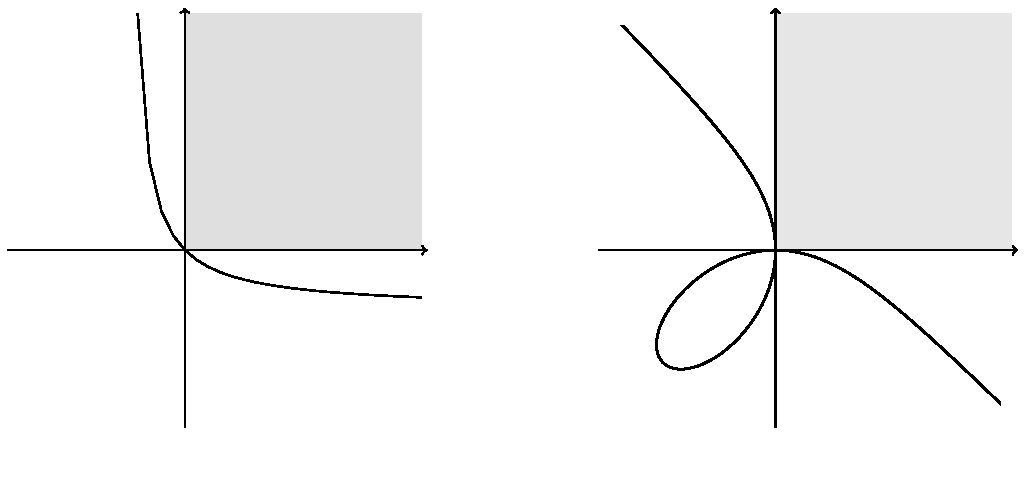
\includegraphics[scale=0.75]{fig_1.pdf}
\end{center}
\vspace{-5ex}
\caption{Left: $p=x+y+xy$, Right: $p=x^3+y^3+xy$}
\label{fig_1}
\end{figure}

The main tool used in this article to solve this problem is blowing up (or blow-up).
Briefly speaking, blow-up (along the original point) introduces additional dimensions for the original point such that
curves crossing it in different directions are lifted to new curves intersecting the additional dimensions in different points.

% In mathematics, blowing up or blowup is a type of geometric transformation which replaces 
% a subspace of a given space with all the directions pointing out of that subspace.
Let's first consider a simple but heuristic example of blowing up. 
Suppose there's a family of line $\{l_i: a_ix+b_iy=0\}_{i=1,\dots,n}$ on the plane 
$\mathbb R^2$
crossing the original point $(0,0)$. 
% The point $(0,0)$ is the common zero set of these lines,
% however it only contains little information of these lines. In another viewpoint,
% $(0,0)$ is a `singularity' because generally $n$ lines cannot cross each other 
% at a common point on the plane. 
If we want know how these lines cross the point $(0,0)$, we can introduce 
new variables $u$, $v$ and $t$ such that
\[
	x=ut,\quad y=vt,
\] 
where $[u:v]$ is a projective coordinate, since any common factor of $u$ and $v$ can be absorbed into the definition of $t$, the line $l_i:a_ix+b_iy=0$ hence becomes a line parameterized 
by $t$ with an additional point $[-b_i:a_i]\in \mathbb P^1$. These additional points in $\mathbb P^1$ tell us how these line approach $(0,0)$ so that they can be used to distinguish different lines.
In other words, we replace the point $(0,0)$ with $\mathbb P^1$, which is the additional dimension mentioned above. 

% Now Let us see how blowing up resolves singularities. 
% Consider the curve $x^3+y^3+xy=0$ on the plane, which is drawn in Fig.\ref{fig_1}.
% It crosses the original point twice in different 
% directions. Therefore, after blowing up, the uplifted curve intersects $\mathbb P^1$ with two 
% different points so that it has no self-intersection. 

The above example is called the blow-up of the plane along the original point.
In this article, we will consider the blow-up of $\mathbb R^D$
along subspace $\mathbb R^n$ defined by $x_{i_1}=\cdots=x_{i_n}=0$. 
The blow-up is the variety defined by equations $\{x_{i_j}y_k=x_{i_k}y_j\,:\, 1\leq j<k\leq n\}$ in space 
$\mathbb R^{D}\times \mathbb P^{n-1}$,
where $[y_1:\dots:y_n]$ is the projective coordinate. 
%These equations can be easily solved by 
%$x_{i_j}=ty_{j}$ for $t\neq 0$.

% Generally, let $X=\operatorname{Spec} A$ be an affine scheme, and let $V(f_1,\dots,f_n)\subset X$
% is a closed subscheme of $X$. The blow-up of $Y$ in X is the closure in
% $X\times_A \mathbb P_A^{n-1}=\mathbb P_A^{n-1}$ of the graph of the morphism 
% \[
% \alpha_{(f_1,\dots,f_n)}:X-Y\to \mathbb P_A^{n-1}.
% \] 

Now let's carefully consider the first example, the integral \eqref{exam:1}
\[
	I=\int_0^\infty \int_0^\infty\frac{dx}{x}\frac{dy}{y}x^{\alpha' a}y^{\alpha' b}(x+y+x y)^{-\alpha' c},
\]
whose leading contribution comes from the neighbourhoods of four vertices $(0,0)$, $(0,\infty)$, $(\infty,0)$ and $(\infty,\infty)$. One can easily see that the vertices $(0,\infty)$, $(\infty,0)$ and $(\infty,\infty)$ are normal crossing. The consequence of this fact is the integrand decouples into powers of $x$ and $y$, then the leading contribution can be trivially obtained, for example 
\begin{align*}
	I(0,\infty)&=\int_{0}^\epsilon\int_{1/\epsilon}^\infty \frac{dx}{x}\frac{dy}{y}x^{\alpha' a}y^{\alpha' b}(x+y+xy)^{-\alpha' c} \\
	&\approx \int_{0}^\epsilon\int_{1/\epsilon}^\infty \frac{dx}{x}\frac{dy}{y}x^{\alpha' a}y^{\alpha' (b-c)}= 
	\frac{1}{{\alpha'}^2}\frac{1}{a} \frac{1}{c-b}+O({\alpha'}^{-1}),
\end{align*}
where we throw away $x$ and $xy$ in $x+y+xy$ after $\approx$ because in this case $x\ll y$
so that they do not contribute the leading order when $\alpha' \to 0$.
In this article, the symbol $\approx$ is used to relate two expressions 
(usually integrals) with the same leading terms 
or two polynomials which contribute the same leading terms in the integration.
Similarly, $I(\infty,0)\approx ({\alpha'}^2 b (c-a))^{-1}$ and $I(\infty,\infty)\approx (\alpha'^{2}(c-a) (c-b))^{-1}.$

The vertex $(0,0)$ is harder due to the behaviour of the mixed factor $(x+y+xy)^{-\alpha' c}$ at the neighbourhood of this vertex. 
% \[
% I(0,0)=\int^{\epsilon}_0 \int^{\epsilon}_0 \frac{dx}{x}\frac{dy}{y}x^{\alpha' a}y^{\alpha' b}(x+y+xy)^{-\alpha' c}
% %\sim\int^{\epsilon}_0 \int^{\epsilon}_0\frac{dx}{x}\frac{dy}{y}x^{\alpha' a}y^{\alpha' b}(x+y)^{-\alpha' c}.
% \]
% when $(x,y)\to (0,0)$, we cannot decouple $x$ and $y$ in the mixed factor $(x+y+xy)^{-\alpha' c}$ 
% because we don't know which one is dominated. 
However, we can always drop the term $xy$ which becomes irrelevant 
when $(x,y)\to (0,0)$ because $xy\ll x$, $y$. 
For remaining terms $x+y$, 
we blow up the plane along $(0,0)$ by introducing new variables 
$(t,[u:v])$ defined by equations $x=tu$ and $y=tv$ in
$\mathbb R\times\mathbb P^1$. 
Because $x$, $y\geq 0$ in the integral region,
%It's convenient to further identify the $\mathbb P^1$ with
%the line $u+v=1$ defined in $\mathbb R^2$.
the vertex $(0,0)$ is blown up to an one-dimensional simplex $\mathbb P^1_+=\{[u:v]\,:\,u,v\geq 0\}$ 
with two new vertices $u=0$ and $v=0$ under this map, 
and it is easy to see that the factor $(x+y)$ is dominated by $x$ near the vertex $u=0$ or 
by $y$ near the vertex $v = 0$. More precisely,
the one-dimensional simplex $\mathbb P^1_+$ can be identified with 
the unit interval $[0,1]$ by setting $u+v=1$, so
 \begin{equation}\label{canonicalformunderblowup}
	\frac{dxdy}{xy} = \frac{du}{u(1-u)}\frac{dt}{t},
 \end{equation}
and
\begin{equation*}
	I(0,0)\approx\int_0^\epsilon\frac{dt}{t} t^{\alpha'(a+b-c)}\int_0^{1}\frac{du}{u(1-u)}u^{\alpha' a}(1-u)^{\alpha' b}%\sim \frac{1}{\alpha'}\frac{1}{a+b-c}\int_0^{1}\frac{dp}{p(1-p)}p^{\alpha' a}(1-p)^{\alpha' b}
	= \frac{1}{{\alpha'}^2}\frac{1}{a+b-c}\biggl(\frac 1a+\frac 1b\biggr)
	+O({\alpha'}^{-1}).
\end{equation*}
% In this example, whether $x$ or $y$ is dominated in the integration is characterized by $p$, 
% and both vertices $p\approx 0$ ($x\ll y$) and $p\approx 1$ ($y\ll x$) contribute.
\begin{center}
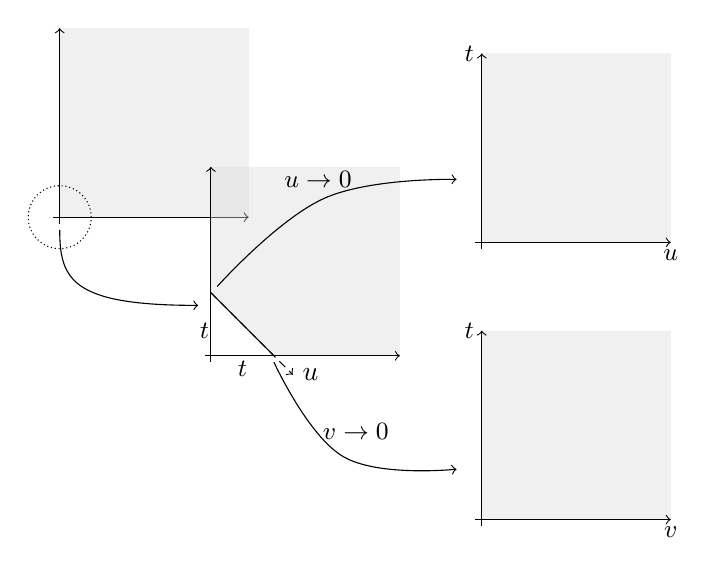
\begin{tikzpicture}[scale=0.8]
\fill[gray!30,opacity=0.4] (-6.9,1.4) -- (-3.9,1.4) -- (-3.9,4.4) -- (-6.9,4.4);
\draw[->] (-7,1.4) -- (-3.9,1.4);
\draw[->] (-6.9,1.3) -- (-6.9,4.4);
\draw[densely dotted]  (-6.9,1.4) ellipse (0.5 and 0.5);
\draw[->] (-6.9,1.2) .. controls (-6.9,0.4) and (-6.7,0) .. (-4.7,0);
\fill[gray!30,opacity=0.4] (-3.5,-0.8) -- (-1.5,-0.8) -- (-1.5,2.2) -- (-4.5,2.2) -- (-4.5,0.2);
\draw[->] (-4.6,-0.8) -- (-1.5,-0.8);
\draw[->] (-4.5,-0.9) -- (-4.5,2.2);
\draw (-3.5,-0.8) -- (-4.5,0.2);
\draw[densely dashed,->] (-4.5,0.2) -- (-3.2,-1.1)node[right]{$u$};
\draw[->]  plot[smooth, tension=.7] coordinates {(-4.4,0.3) (-2.7,1.7) (-0.6,2)};
\draw[->]  plot[smooth, tension=.7] coordinates {(-3.5,-0.9) (-2.4,-2.4) (-0.6,-2.6)};
\fill[gray!30,opacity=0.4] (0.8,-3.4) -- (2.8,-3.4) -- (2.8,-0.4) -- (-0.2,-0.4) -- (-0.2,-3.4);
\draw[->] (-0.3,-3.4) -- (2.8,-3.4);
\draw[->] (-0.2,-3.5) -- (-0.2,-0.4);
\fill[gray!30,opacity=0.4] (0.8,1) -- (2.8,1) -- (2.8,4) -- (-0.2,4) -- (-0.2,1);
\draw[->] (-0.3,1) -- (2.8,1);
\draw[->] (-0.2,0.9) -- (-0.2,4);
\node at (-2.8,2) {\small $u\to 0$};
\node at (-2.2,-2) {\small $v\to 0$};
\node at (-4,-1) {\small $t$};
\node at (-4.6,-0.4) {\small $t$};
\node at (2.8,0.8) {\small $u$};
\node at (-0.4,4) {\small $t$};
\node at (-0.4,-0.4) {\small $t$};
\node at (2.8,-3.6) {\small $v$};
\end{tikzpicture}
\end{center}
% Similarly, one can work out 
% \[
% 	I(\infty,\infty)\approx \frac{1}{{\alpha'}^2}\frac{1}{(c-a) (c-b)} 
% \]
% and 
Finally,
\begin{align*}
	I&\approx I(0,0)+I(0,\infty)+I(\infty,0)+I(\infty,\infty)\\
	 &\approx \frac{1}{{\alpha'}^2}
	 \biggl(
\frac{1}{b (a+b-c)}+\frac{1}{b (c-a)}+\frac{1}{a (c-b)}+\frac{1}{(c-a) (c-b)}+\frac{1}{a (a+b-c)}
	 \biggr).
\end{align*}
%similarly, 
%\[
%	I(\infty,\infty)\sim \frac{1}{{\alpha'}^2}\frac{1}{c-a-b}\biggl(\frac 1{c-a}+\frac 1{c-b}\biggr),
%\]
%so the leading terms of original integral is 
%\[
%	I\sim I(0,0)+I(0,\infty)+I(\infty,0)+I(\infty,\infty).
%\]



From the last example, we can see that polynomials are not canonical objects 
for the leading order of a integral because different polynomials can give the 
same contribution. For example, we can throw away irrelevant terms in the 
polynomial. Besides, the integral also doesn't depend on positive coefficients
in the polynomial which we will explain later.
Thus a natural question arises. What's the canonical object to describe the 
leading contribution of a polynomial in a integral near a vertex? The answer is 
the \textit{Newton polyhedron} of this polynomial.

\begin{defi}[Newton polyhedron]
Let $p=\sum_{I}s_I x^{n^I}$ be a polynomial with positive coefficients.
For each term $s_I x^{n^I}$, we assign a cone 
$C_{I}=(n^I+\mathbb R^D_{+}):=\{(n^I_1+v_1,\dots,n^I_D+v_D)\,:\, 
\text{$v_i\geq 0$ for all $i$}\}$. The 
\textit{Newton polyhedron} $C[p]$ of the polynomial $p$ 
is the \textit{convex hull} of cones $\{C_I\}$, 
\textit{i.e.} the smallest convex set contains these cones.
\end{defi}

Note that the Newton polyhedron of $p$ doesn't depend on
positive coefficients $s_I$.

%Concretely, suppose we come to the vertex defined locally by $x_1=\cdots=x_D=0$, 
%and consider the integral
%\[
	%I(0,\dots,0)=\int_{[0,\epsilon]^D} 
	%\biggl(\prod_{i=1}^D\frac{d x_i}{x_i}x_i^{\alpha' X_i}\biggr)
	%p(x)^{-\alpha'c}\prod_a(q_a(x))^{-\alpha' c_a}.
%\]

%It's usually larger than the union of these cones $\bigcup_I C_I$, 
%but terms other than vertices of the Newton polyhedron 
%also doesn't contribute! 
%Here let's consider an example $p(x)=x^6+y^6+x^2y^2$. 
%\begin{center}
	%\begin{tikzpicture}
		%\fill[gray,opacity=0.2] (0,4) -- (0,3) -- (4,3) -- (4,4);
		%\fill[gray,opacity=0.2] (1,4) -- (1,1) -- (4,1) -- (4,4);
		%\fill[gray,opacity=0.2] (3,4) -- (3,0) -- (4,0) -- (4,4); 
		%\fill[green,opacity=0.2] (0,3) -- (1,3) -- (1,1); 
		%\fill[green,opacity=0.2] (3,0) -- (3,1) -- (1,1); 
		%\draw[thick] (0,4) -- (0,3) -- (1,1) -- (3,0) -- (4,0);
		%\draw[->](-0.1,0) -- (4.1,0);
		%\draw[->](0,-0.1) -- (0,4.1);
		%\node[inner sep=1.5pt,circle,fill=blue] at (0,3) {};
		%\node[inner sep=1.5pt,circle,fill=blue] at (1,1) {};
		%\node[inner sep=1.5pt,circle,fill=blue] at (3,0) {};
	%\end{tikzpicture}
%\end{center}
%In the above diagram, besides gray cones, the polyhedron contains two green regions. 
%If we add terms like $x^5y^2$ in the interior of green regions to the polynomial, 
%we will show in the next lemma that the leading terms of the integral 
%from this vertices $x_1=x_2=\cdots=x_D=0$ do not change.

\begin{pro}
The leading order of integrals
\[
	I=\int_{[0,\epsilon]^D} \left(\prod_{i=1}^D\frac{\dif x_i}{x_i}x_i^{\alpha' X_i}\right)
	p^{-\alpha' c} \prod_a q_a^{-\alpha' c_I}
\]
only depends on the Newton polyhedron $C[p]$.
\end{pro}

From the theorem in \cite{Arkani-Hamed:2019mrd}, the leading order of the integral eq.\eqref{int1} 
only depends on the Minkowski sum of Newton polytopes of polynomials $p_I$.
The \textit{Newton polytope} of a polynomial is very like the Newton polyhedron of a polynomial defined above.
For a polynomial $q=\sum_I a_I x^{n^I}$, it's the convex hull of vectors 
$\{n^I=(n^I_1,\dots,n^I_D)\}$. The
\textit{Minkowski sum} (or vector sum) of two set $A$ and $B$ is the set $\{x+y\,:\,x\in A,\,y\in B\}$. 
Note that the Newton polyhedron of a polynomial is just the Minkowski sum of Newton polytope and $\mathbb R_+^D$.

Therefore, the above proposition is like the local version of this theorem, 
so it may seem trivial. However, it's more free to use the local version because 
the cone is not as rigid as the Newton polytope, and it just looks  
like a `corner' of the Newton polytope.

%\begin{lem}
%Suppose $p(x)=\sum_{I\in \mathscr A}a_I x^{n^I}$ is a polynomial, and $C[p]$ is the convex hull
%of cones $\{C_{I}=(n^I+\mathbb R^D_{+})\}$. 
%When we consider the integral near the vertices $x_1=\cdots=x_D=0$, 
%then we can replace $p(x)$ by a new polynomial $\bar p(x)=\sum_{J\in \mathscr B}a_J x^{n^J}$ such that
%the leading order of the integral does not change.
%\end{lem}

% In the following proof, we define $|v|=\sum_{i=1}^D v_i$ for any vector $v\in \mathbb R^D$.

\begin{proof}
Suppose $p=\sum_I s_I x^{n^I}$.
We first prove that the integral doesn't depend on 
positive coefficients $\{s_I\}$.
In fact, if $x^{n^I}$ dominates $p$ in the limit process $\mathcal L$, 
then the contribution of integral from this process is
\begin{align*}
	\int_{\mathcal L} 
	\biggl(\prod_{i=1}^D\frac{d x_i}{x_i}x_i^{\alpha' X_i}\biggr)
	p(x)^{-\alpha'c}\prod_a(q_a(x))^{-\alpha' c_a}
	&\approx s_I^{-\alpha' c}
	\int_{\mathcal L} 
	\biggl(\prod_{i=1}^D\frac{d x_i}{x_i}x_i^{\alpha' X_i-\alpha' cn^I_i}
	\biggr)\prod_a(q_a(x))^{-\alpha' c_a},
\end{align*}
but $s_I^{-\alpha' c}=1+O(\alpha')$ doesn't affect its leading terms.

Nest we prove that terms in the Newton polyhedron can be dropped in the 
integration.
For a term $x^{n^J}\neq x^{n^I}$ in the cone $C_I$, we should get that
$n^J_i\geq n^I_i$ for every $i$, then there's no need to consider 
$x^{n^J}$ anymore because it goes to zero faster than $x^{n^I}$. Thus
terms other than vertices in $\bigcup_I C_I$ do not contribute. 

Suppose a term $x^v$ is in the interior of $C[p]-\bigcup_I C_I$,  
then there exist non-negative numbers $\{c_J\}$ such that it can be written as 
\[
	v = \sum_{J\in \mathscr B}c_J n^J,\quad \sum_{J\in \mathscr B} c_J>1.
\]
If $x^{n^L}$ dominates some limit process, 
then for other $J\in \mathscr B$, there exists a non-negative number $r_J$ such that
$x^{w^J}:=x^{n^L-n^J}\leq r_J$, then 
\[
	x^v = \prod_{J\in\mathscr B} (x^{n_J})^{c_J} = 
	(x^{n_L})^{\sum_J c_J}\prod_{J\in \mathscr B} 
	(x^{w_J})^{c_J}\leq R\,(x^{n_L})^{\sum_J c_J}
\] 
where $R$ is a non-negative number and $\sum_J c_J>1$, so $x^v$ goes to 
zero faster than $x^{n_L}$. Since $L\in \mathscr B$ is arbitrary, $x^v$ can be thrown away.

Finally, suppose that $v$ is on the boundary of $C[p]$ but not a vertex.
% then it can be written as 
% \[
% 	v = \sum_{J\in \mathscr C}c_J n^J,\quad \sum_{J\in \mathscr C} c_J=1,
% \]
% where $\mathscr C$ is the set of vertices on the same boundary as $v$.
We can prove the result by showing this terms goes to zero faster than some vertices on the 
same boundary, so we can further assume that $p$ is a homogeneous polynomial.
After blowing-up, near the new vertex
$y_i=1$, the polynomial becomes $p'=t^{\sum_i v_i}\sum_{I}a_I y^{n^I}|_{y_i=1}$. 
Since $v$ is not a vertex, it should be in the interior of the polyhedron of this new polynomial or 
on the boundary of the polyhedron (for all $i$), and then by 
the proven part of lemma and induction on codimension, it doesn't contribute the integral.
\end{proof}

% Geometrically, if we consider the cone $C$ spanned by all $\{n^I\}$, then the basis can be choosen as the vertices on the boundary of $C$, and terms corresponding to points inside $C$ can be dropped.
% For example, suppose that $p(x,y)=x^3+y^3+xy+x^3y^2+xy^3$, we draw each $n^I$ in the following diagram,
% \begin{center}
% 	\begin{tikzpicture}
% 		\fill[gray!20] (0,4) -- (0,3) -- (1,1) -- (3,0) -- (4,0) -- (4,4);
% 		\draw[thick] (0,4) -- (0,3) -- (1,1) -- (3,0) -- (4,0);
% 		\draw[->](-0.1,0) -- (4,0);
% 		\draw[->](0,-0.1) -- (0,4);
% 		\node at (3,2) {$\times$};
% 		\node at (3,1.5) {$x^3y^2$};
% 		\node at (1,3) {$\times$};
% 		\node at (1,2.5) {$xy^2$};
% 		\node[inner sep=1.5pt,circle,fill=blue] at (0,3) {};
% 		\node[inner sep=1.5pt,circle,fill=blue] at (1,1) {};
% 		\node[inner sep=1.5pt,circle,fill=blue] at (3,0) {};
% 	\end{tikzpicture}
% \end{center}
% where $x^3y^2\leftrightarrow (3,2)$ and $xy^3\leftrightarrow (1,3)$ are represented by $\times$ in the diagram and other terms are represented by blue points. The basis is given by blue points $\{x^3\leftrightarrow (3,0),y^3\leftrightarrow (0,3),xy\leftrightarrow (1,1)\}$, and the gray region is the set of all vectors $v=\sum_{J\in \mathscr B}c^I_J n^J$ where $\sum_J c^I_J>1$, therefore we throw away terms in the gray region and then get that $\bar p(x)=x^3+y^3+xy$. 

By using the language of the polyhedron of a polynomial $p$, the goal of blowing up is clear.
If one gets polyhedron of a polynomial $p$ like
\begin{center}
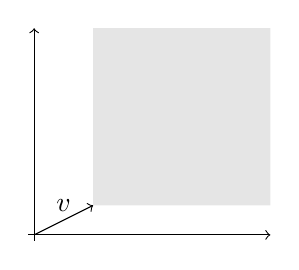
\begin{tikzpicture}[scale=0.75,baseline={([yshift=-.5ex]current bounding box.center)}]
\fill[gray!20] (2,3) -- (0,3) -- (0,0) -- (3,0) -- (3,1) -- (3,3);
\draw[->](-1.1,-0.5) -- (3,-0.5);
\draw[->](-1,-0.6) -- (-1,3);
\draw[->] (-1,-0.5) -- (0,0);
\node at (-0.5,0) {$v$};
\end{tikzpicture}
\end{center}
then we call that $p\approx x^v$ is decoupled. In other words, $p$ has the form of 
\(
p(x)=x^v(c+q(x))
\) for a vector $v$ and polynomial $q$ with $q(0)=0$. 
Suppose $p\approx x^v$ is a decoupled polynomial, then
the integral
\[
	I=\int_{[0,\epsilon]^D} \left(\prod_{i=1}^D\frac{\dif x_i}{x_i}x_i^{\alpha' X_i}\right)
	p^{-\alpha' c} \prod_I q_I^{-\alpha' c_I}
	\approx\int_{[0,\epsilon]^D} \left(\prod_{i=1}^D\frac{\dif x_i}{x_i}x_i^{\alpha' (X_i-cv_i)}\right)
	\prod_I q_I^{-\alpha' c_I},
\] 
is reduced to a new integral with less polynomials but with the same leading order. 
Since blow-ups never increase the 
number of the polynomial in the integral, we only need to consider the integrals with only one 
polynomial
\[
	I=\int_{[0,\epsilon]^D} \left(\prod_{i=1}^D\frac{\dif x_i}{x_i}x_i^{\alpha' X_i}\right)
	p^{-\alpha' c}.
\] 
Our aim is to find a series of blow-ups to make this polynomial $p$ decoupled at
each generated vertices.

After declaring the aim of blow-ups by the language of polyhedra, 
it's a good time to consider general blow-ups and see what they do on integrals and polyhedra.

As hinted by eq.\eqref{canonicalformunderblowup}, one important feature of $\Omega_{\mathcal P}$
is `invariant' under the blowing-up because the residue of the canonical form on the boundary is
the canonical form of the boundary.
Suppose we blow up near the boundary defined locally by $x_1=\cdots=x_n=0$ in integral eq.\eqref{int1}. 
It's already the most general cases. In fact, if in the definition of a boundary $x_i=\infty$, we can
change the variable $x_i\mapsto 1/x_i$ and then $x_i=0$.
Let $x_i=ty_i$, where $[y_1:\dots:y_n]$ are positive projective coordinates. 
Near the boundary, the canonical form of $\Omega$ performs as 
\[
	\Omega=\frac{dx_1}{x_1}\wedge \cdots\wedge\frac{dx_n}{x_n}
	\wedge \Phi(x'),
\]
where $x'$ are other coordinates. In new coordinates, it can be written as 
\[
	\Omega=\frac{1}{y_n}\frac{dt}{t}\wedge \frac{dy_1}{y_1}\wedge \cdots
	\wedge\frac{dy_{n-1}}{y_{n-1}}\wedge \Phi(x')+O(t^0),
\]
where $y_n=1-(y_1+\cdots+y_{n-1})$ and $\Phi$ is the canonical form of the boundary of $\mathcal P$ given by $x_1=\cdots=x_n=0$. Therefore,
\[
	\operatorname{Res}_{t=0}(\Omega)=\frac{1}{y_n}\frac{dy_1}{y_1}\wedge \cdots\wedge\frac{dy_{n-1}}{y_{n-1}}\wedge \Phi(x')=\Omega_{n-1}(y)\wedge \Phi(x'),
\]
$\Omega_{n-1}(y)$ the canonical form of a standard $(n-1)$-dimensional simplex $\mathbb P^{n-1}_+$ defined by
$
	\sum_{i=1}^n y_i=1
$ and $y_i\geq 0$. 
% If we rewrite it in new coordinates $\{z_i\}$ such that
% \[
% 	z_0=0,\quad y_i=z_i-z_{i-1},\quad z_{n}=1,
% \]
% then 
% \[
% 	\Omega_{n-1}(z)=\frac{dz_1\wedge\cdots\wedge dz_n}{(z_1-z_0)\cdots (z_n-z_{n-1})}.
% \]
% It's the more familiar form.

% Consider a set of irreducible polynomials $\{p_i\}$, let $Z(p_i)$ be the zero point set of $p_i$ in $\mathbb{R}^n$. Suppose a curved polytope $\mathcal P$ is bounded by $\bigcup_i Z(p_i)$, if $F_k$ is a codimension $k$ face of $\mathcal P$ where $\#\{i\,:\,F_k\subset Z(p_i)\}>k$, then we call it a degenerated face.

% Now Consider the integration
% \[
% 	I(\alpha')=\int_{\mathcal P} \Omega_{\mathcal P}(x)\prod_i(p_i(x))^{\alpha' s_i},
% \]
% where $\Omega$ is the canonical form of $\mathcal P$, and we suppose $I(\alpha')$ is finite when $\alpha'>0$.
% It's clear that $I(\alpha')$ diverge when $\alpha'\to 0$. We want to find all possible poles in the leading order of its Laurent series with respect to $\alpha$ at $\alpha=0$. It's a rational function of $s_i$ since $p_i$ are all polynomials.

% If $F$ is a facet of $\mathcal P$. Locally, if $F$ is defined by $x=0$, then near $F$, the integration is 
% \[
% 	\int_0^\epsilon \frac{d x}{x} x^{\alpha' a} \int_{x'}\Psi(x')
% 	\sim \frac{1}{\alpha' a}\int_{x'}\Psi(x'),
% \]
% where $x'$ are other coordinates and $\Psi(x')$ is the left part of $\Omega_{\mathcal P}(x)\prod_i(p_i(x))^{\alpha' s_i}$.

% For polynomials, suppose that 
% $p_i(x) = t^{k_i}q_i(x',y,t)$.
% then the integral eq.\eqref{int1}, near this boundary and when $\alpha'$ is small, becomes
% \[
% \begin{aligned}
% \int_{x'} \int_{x\in [0,\epsilon]^n} \Omega(x,x')\,\prod_ix_i^{\alpha' X_i}&
% \prod_i(p_i(x))^{-\alpha' c_i}=
% \int_0^\epsilon \, \frac{dt}{t} t^{\alpha'\sum_{i=1}^n X_i-\alpha' \sum_I k_Is_I}\\
% 	  &\int_{y\in\delta_{n-1}}\Omega_{n-1}(y)
% \prod_{j=1}^n y_j^{\alpha' x_j}
% \int_{x'}\phi(x')\prod_{k=n+1}^D(x'_k)^{\alpha' X_k}
% \prod_i(q_i(x',y,t))^{-\alpha' c_I},
% \end{aligned}
% \]
% however we still need to worry about the blowing-up of $t$, $y$ and $x'$ in $q_I$ because
% it's still unknown that which one is dominated.

Another important feature of the canonical form is about the rescale of exponents of variables.
If we change the variables by
\(
	x_i\mapsto x_i^{1/c_i}
\)
for $i\in S$, where $c_i$ is a positive rational number, then integral becomes
\[
	\prod_{i\in S}c_i\int
	\prod_{j\not\in S}\frac{\dif x_j}{x_j}x_j^{\alpha' X_j}
	\prod_{i\in S}\frac{\dif x_i}{x_i}x_i^{\alpha' c_iX_i}
	p(\{x_i^{c_i}\,:\, i\in S\};\{x_j\,:\, j\not\in S\})^{-\alpha' c}.
\]
Note that the rescale of the integral region doesn't change the leading order of the integral
because $\epsilon^{\alpha'}$ and $(\epsilon^{1/c_i})^{\alpha'}$ both behave as $1+O(\alpha')$
when $\alpha'\to 0$. Thus, it only introduces a factor $\prod_{i\in S}c_i$ 
for the integral and doesn't break the form of the integral 
thanks to $\dif \log$ singularities of the canonical form.

Blowing up produces new vertices 
$
	\{v_i:x'=0,t=0,y_i=1\}
$.
Note that $y_i=1$ means that $y_j=0$ for $j\neq i$ because $\sum_i y_i=1$. 
Therefore, it's equivalent to do such change of variables
\[
	x'\to x',\quad x_j\to ty_j\quad \text{for $j\neq i$},\quad x_i\to t,
\]
or by reusing the name of $x_i$ for $t$ and $x_j$ for $y_j$ to save the namespace,
\[
	x_j\to x_ix_j\quad \text{for $j\neq i$}.
\]
% which is related to the sector decomposition. 
% We will use this change of variable from now on.
In terms of this change of variables, the polynomial $p=\sum_I a_I x^{n^I}$ becomes 
$p'=\sum_I a_I x^{(n^I)'}$, where
\[
	(n^I)'_i\longrightarrow \sum_j n^I_j,
\]
and it can be visualized by the polyhedron.
For example, for $p(x)=x^3+xy+y^3$, the gray polyhedron, we first get the green polyhedron, 
but it's not the wanted (decoupled) polyhedron, so we blow up it again and we get the red polyhedron.
\begin{center}
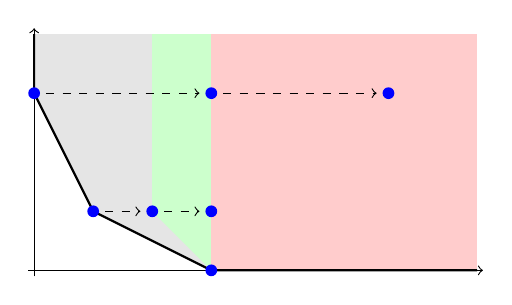
\begin{tikzpicture}[scale=0.75]
	\fill[gray!20] (0,4) -- (0,3) -- (1,1) -- (3,0) -- (4,0) -- (7.5,4);
	\fill[green!20] (2,4) -- (2,1) -- (3,0) -- (4,0) -- (7.5,4) --cycle;
	\fill[red!20] (3,4) -- (7.5,4) -- (7.5,0) -- (3,0)-- cycle;
	\draw[thick] (0,4) -- (0,3) -- (1,1) -- (3,0) -- (7.5,0);
	\draw[->](-0.1,0) -- (7.6,0);
	\draw[->](0,-0.1) -- (0,4.1);
	\node[inner sep=1.5pt,circle,fill=blue] at (0,3) {};
	\node[inner sep=1.5pt,circle,fill=blue] at (1,1) {};
	\node[inner sep=1.5pt,circle,fill=blue] at (3,0) {};
	\node[inner sep=1.5pt,circle,fill=blue] at (2,1) {};
	\node[inner sep=1.5pt,circle,fill=blue] at (3,3) {};
	\node[inner sep=1.5pt,circle,fill=blue] at (3,1) {};
	\node[inner sep=1.5pt,circle,fill=blue] at (6,3) {};
	\draw[dashed,->] (0.2,3) -- (2.8,3);
	\draw[dashed,->] (1.2,1) -- (1.8,1);
	\draw[dashed,->] (3.2,3) -- (5.8,3);
	\draw[dashed,->] (2.2,1) -- (2.8,1);
\end{tikzpicture}
\end{center}
Note that we still need to work out other vertices generated by blow-ups. 

However, usually a bad choice of set of variables to blow up may lead to the
infinite recursion in higher dimension.
For example, 
\[
	p(x_1,x_2,x_3)=x_1x_3^2+x_2^2+x_2x_3,
\]
if we choose $x_1$ and $x_2$ to blow up, then for the vertex 
$\{x_1\mapsto x_1, x_2\mapsto x_1x_2, x_3\mapsto x_3\}$,
\[
	p(x_1,x_2,x_3)\mapsto x_1(x_1x_2^2+x_3^2+x_2x_3)=x_1 p(x_1,x_3,x_2).
\]
We will get the polynomial $p$ again and then an endless loop if we always choose such
variables to blow up.

Therefore, a natural question arises. For a given polynomial $p$, 
can we terminate after finite steps such that near each generated vertex, $p$ becomes 
decoupled? This question is first declared by Hironaka \cite{hironaka1967}. 
He designed a game to describe this question, which is 
called Hironaka's polyhedra game. Let's recall the game rule in our language.

Suppose $p$ is a given polynomial. There are two players A and B in the game. 
At each round, first A choose a set of variables $\{x_{i_1},\dots,x_{i_n}\}$, then
B choose one variable $x_{i_k}$ out of them and make variable substitutions
$x_{i_j} \to x_{i_k}x_{i_j}$ for $j\neq k$.
If $p$ becomes decoupled, then player A wins, otherwise they start a new round by using the 
new generated polynomial. If player A cannot win in finite rounds, player B wins.

%How to win this game is equivalent to how to resolve singularities
%by a series of blow-ups, \textit{i.e.}
%a winning strategy for player A is a construction of resolution of singularities. 

It's clear that any winning strategy for player A will tell us how to 
calculate stringy integrals. There're many know winning strategies.
\cite{spivakovsky1983solution,zeillinger2006short,hauser2003hironaka}
However, they are not so efficient. ... 
% [Spivakovsky 83], [Encinas \& Hauser 02], [Zeillinger 05], \dots.

% We mainly use the Zeillinger's method in the calculation. 
% It's not the most efficient one, but it can be understood well by the picture of 
% polyhedron. Let's give a quick review here.
% 
% Let's start from a polyhedron $C[p]$. The vertices set of $C[p]$ is denoted by $M_p$. After
% blowing-up, they becomes $C[p']$ and $M'_p$. First note that $|M'_p|\leq |M_p|$ because
% the shift (blowing-up) can only keep a vertex or move it into the convex hull. Next note
% that if $|M_p|=1$, then $p$ is decoupled. Therefore, a possible winning strategy for player
% A is to find a set of variables to blow up at each round such that $|M_p|$ strictly decreases.
% However, it's usually too far for a winning strategy to satisfy this condition. Therefore,
% we need to add more elaborate conditions, \textit{e.g.} 
% the number of variables of non-decoupled part of polynomial. At each round, we only need 
% that one of these numbers strictly decreases. Zeillinger designed a triple of such numbers
% in the following way.
% 
% For a polynomial $p$, define the set
% \[
% 	W[p]=\{n^I-n^J\,:\, I,J\in \mathscr B\},
% \]
% where $\mathscr B$ is the set of vertices of $C[p]$. After blowing-up, $(n^I)'$ doesn't 
% need to be a vertex, but we still can talk about the image of $W[p]$ of blowing-up.
% Note that $p'$ is decoupled if and only if for any $v$ in the image of $W[p]$, 
% $v\in \mathbb Z_{\geq 0}^D$ or $v\in \mathbb Z_{\leq 0}^D$.
% Furthermore, we define the gap function for any $v\in W[p]$
% \[
% 	g(v)=\max_i v_i-\min_i v_i 
% \]
% to be the difference of maximum and minimum of $v$, and
% \[
% 	l(v)=\#\{j\,:\, v_j=\max_i v_i\}+\#\{j\,:\, v_j=\min_i v_i\},
% \] 
% which counts how many times do components of $v$ take the minimum or maximum. 
% 
% Now for a polynomial $p$,
% find the minimal element $v\in W[p]$ with respect of the lexicographical ordering of
% tuple $(g(v),l(v))$, then player A chooses variables $\{x_r,x_s\}$, where $r$ and $s$ are 
% defined by
% \[
% 	v_r=\min_i v_i\quad \text{and}\quad v_s=\max_i v_i.
% \]
% Denote the minimal element by $(G,L)=(g(v),l(v))$. 
% The triple designed by Zeillinger is $(|M_p|,G,L)$. We will not go into details of the proof. 


\section{Application and Example}

% string Z integral, Cn, Gkn ...
In this section, we will give several examples to illustrate this blow-up method, all examples comes from the so-called cluster stringy integrals~\cite{} which are closely related to the origin string integrals. The dimension of all examples in this section is 2 or 3 and the regulating polynomials are simple, so the blow-up prescriptions can be designed \emph{ad hoc} without a universal algorithm.


\subsubsection*{Cluster string integral: $A_{2}$}
This integral is equivalent to the $Z$-integral $Z_{12345}(1,2,3,4,5)$~\cite{}, which in a positive parameterization takes the form of 
\[
	\mathcal{I}_{A_{2}}=\int_{\mathbb R_+^2} \frac{\dif x_1}{x_1}\frac{\dif x_2}{x_2}x_1^{\alpha' X}x_2^{\alpha' Y}
	(1+x_1)^{-\alpha' a}(1+x_2)^{-\alpha' b}(1+x_1+x_1x_2)^{-\alpha' c}
\] 
where $1+x_{1}$, $1+x_{2}$ and $1+x_{1}+x_{1}x_{2}$ are $F$-polynomials with the initial seed $A_{2}$ quiver. With variable substitutions
\[
	x_{1}=\frac{1-z_{3}}{z_{3}}\,,\qquad x_{2}=\frac{z_{3}-z_{2}}{z_{2}(1-z_{3})}
\]
and 
\[
	X=s_{12},\quad Y=s_{45},\quad a=-s_{24},\quad b=-s_{35},\quad c=-s_{25} \:,
	\] 
the integral $\mathcal{I}_{A_{2}}$ becomes $Z_{12345}(12345)$ under the usual gauge fixing $\{z_{1},z_{4},z_{5}\}\to\{0,1,\infty\}$. It is easy to see that vertices $(0,0)$, $(0,\infty)$ and $(\infty,0)$ are all normal crossing, then no blow up is needed and their contributions to leading order simply are
\begin{align*}
	&\mathcal{I}_{A_{2}}(0,0)=\frac{1}{\alpha'^{2}}\frac{1}{XY}+O(\alpha'^{-1}) \:, \\
	%&\mathcal{I}_{A_{2}}(0,\infty)=\frac{1}{\alpha'^{2}}\frac{1}{(a+c-X)Y}+O(\alpha'^{-1}) \:, 
	&\mathcal{I}_{A_{2}}(\infty,0)=\frac{1}{\alpha'^{2}}\frac{1}{(a+c-X)Y}+O(\alpha'^{-1}) \:, \\
	&\mathcal{I}_{A_{2}}(\infty,\infty)=\frac{1}{\alpha'^{2}}\frac{1}{(a+c-X)(b+c-Y)}+O(\alpha'^{-1}) \:.
\end{align*}
The vertex $(0,\infty)$ is not normal crossing, we bring this vertex to the origin by taking $x_{2}\to x_{2}^{-1}$, then the integral over the neighbourhood of this vertex reads
\[
    \mathcal{I}_{A_{2}}(0,\infty) \approx \int_{[0,\epsilon]^{2}} \frac{\dif x_{1}\,\dif x_{2}}{x_{1} x_{2}} x_{1}^{\alpha'X}x_{2}^{\alpha'(b+c-Y)}(x_{1}+x_{2}+x_{1}x_{2})^{-\alpha'c}
\]
where some irrelevant power functions of the form $(1+\cdots)$ have been dropped. This is exactly the example we used in section 2, then the leading order contribution of $\mathcal{I}_{A_{2}}$ is simply
\begin{align*}
   \mathcal{I}_{A_2}&=\frac{1}{\alpha'^{-2}}\biggl(\frac{1}{(a+c-X) (b+c-Y)}+\frac{1}{X (b+X-Y)} \\
   &\quad +\frac{1}{(b+c-Y) (b+X-Y)}+\frac{1}{Y (a+c-X)}+\frac{1}{X Y}\biggr) + O(\alpha'^{-1}) 
\end{align*}

\subsubsection*{Cluster stringy integral: $A_3$}

This integral is equivalent to the $Z$-integral $Z_{123456}(1,2,3,4,5,6)$, which in a positive parameterization takes the form of 
\begin{align*}
	\int_{\mathbb R_+^3} \frac{\dif x_1}{x_1}\frac{\dif x_2}{x_2}\frac{\dif x_3}{x_3}
	x_1^{\alpha' X}x_2^{\alpha' Y}x_3^{\alpha' Z}
	&(x_1 + 1)^{-\alpha' a_1}
	(x_2 + 1)^{-\alpha'a_2}
	(x_3 + 1)^{-\alpha'a_3}
	(x_1x_2 + x_1 + 1)^{-\alpha'a_4}\\
	&(x_2x_3 + x_3 + 1)^{-\alpha'a_5}
	(x_1x_2x_3 + x_1x_3 + x_1 + x_3 + 1)^{-\alpha'a_6}
\end{align*}
where 6 polynomials with constant term 1 are $F$-polynomials with the initial seed $A_{3}$ quiver. With variable substitutions
\[
x_{1}=\frac{(z_{2}-z_{3})(1-z_{4})}{(1-z_{2})(z_{3}-z_{4})}\:,\quad x_{2}=\frac{z_{4}-z_{2}}{z_{2}(1-z_{4})}\:, \quad
x_{3}=\frac{z_{2}}{1-z_{2}}
\]
and
\begin{gather*}
	X=s_{12},\quad Y=s_{123},\quad Z=s_{45} \\
	a_{1}=-s_{24},\quad a_{2}=-s_{36},\quad a_{3}=-s_{15},\quad a_{4}=-s_{26},\quad a_{5}=-s_{35},\quad a_{6}=-s_{25}	
\end{gather*}
the integral $\mathcal{I}_{A_{3}}$ becomes $Z_{123456}(1,2,3,4,5,6)$ under the usual gauge fixing $\{z_{1},z_{5},z_{6}\}\to\{0,1,\infty\}$. Of the 8 vertices, $(0,0,0)$, $(0,0,\infty)$, $(\infty,0,0)$, $(\infty,0,\infty)$ and $(\infty,\infty,\infty)$ are normal crossing ones, and their contributions to leading order is 
\begin{align*}
	\mathcal{I}_{A_{3}}^{(1)}&=\frac{1}{\alpha'^{2}}\biggl(\frac{1}{XYZ}+\frac{1}{F_{1}XY} +\frac{1}{F_{2}YZ}+\frac{1}{F_{1}F_{2}Y} 
	+\frac{1}{F_{1}F_{2}F_{3}}\biggr) +O(\alpha'^{-1})
\end{align*}	
where
\begin{align*}
	F_{1} &= a_{3}+a_{5}+a_{6}-Z \\
	F_{2} &= a_{1}+a_{4}+a_{6}-X \\
	F_{3} &= a_{2}+a_{4}+a_{5}+a_{6}-Y
\end{align*}
For the remaining vertices, we bring them to the origin by setting $x_{i}\to x_{i}^{-1}$,
\begin{align*}
	\mathcal{I}_{A_{3}}(0,\infty,0)&\approx\int_{[0,\epsilon]^{3}}\prod_{i=1}^{3}\frac{\dif x_{i}}{x_{i}} x_{1}^{\alpha' X}
	x_{2}^{\alpha' F_{3}}x_{3}^{\alpha' Z}(x_{1}+x_{2})^{-\alpha' a_{4}}(x_{2}+x_{3})^{-\alpha' a_{5}}
	\biggl(x_{2}+\sum_{i<j} x_{i}x_{j}\biggr)^{-\alpha' a_{6}} \\
	\mathcal{I}_{A_{3}}(\infty,\infty,0)&\approx \int_{[0,\epsilon]^{3}}\frac{\dif x_{i}}{x_{i}}x_{1}^{\alpha' F_{2}}x_{2}^{\alpha' F_{3}}x_{3}^{\alpha'Z} (x_{2}+x_{3})^{-\alpha'(a_{5}+a_{6})} \\
	\mathcal{I}_{A_{3}}(0,\infty,\infty)&\approx \int_{[0,\epsilon]^{3}}\frac{\dif x_{i}}{x_{i}}x_{1}^{\alpha' X}x_{2}^{\alpha' F_{3}}x_{3}^{\alpha' F_{1}} (x_{1}+x_{2})^{-\alpha'(a_{4}+a_{6})}
\end{align*}
where we have dropped some irrelevant terms according to our algorithm. The last two again are the cases we have encountered before, then a further attention is needed only for the first one, which can be decomposed into six normal crossing pieces 
\begin{equation*}
	\mathcal{I}_{A_{3}}(0,\infty,0)\approx
	\begin{cases}
		\int_{[0,\epsilon]^{3}}\prod_{i=1}^{3}\frac{\dif y_{i}}{y_{i}} y_{1}^{\alpha'X} y_{2}^{\alpha' F_{4}}
		y_{3}^{\alpha'F_{5} }  & \{x_{1}=y_{1}y_{2}y_{3}, x_{2}=y_{2}y_{3},x_{3}=y_{3}\} \\
		\int_{[0,\epsilon]^{3}}\prod_{i=1}^{3}\frac{\dif y_{i}}{y_{i}} y_{1}^{\alpha'X} y_{2}^{\alpha' (X+Z)}
		y_{3}^{\alpha'F_{5} }  & \{x_{1}=y_{1}y_{2}y_{3}, x_{3}=y_{2}y_{3},x_{2}=y_{3}\}  \\
		\int_{[0,\epsilon]^{3}}\prod_{i=1}^{3}\frac{\dif y_{i}}{y_{i}} y_{1}^{\alpha' F_{3}} y_{2}^{\alpha' F_{4}}
		y_{3}^{\alpha'F_{5} }  & \{x_{2}=y_{1}y_{2}y_{3}, x_{1}=y_{2}y_{3},x_{3}=y_{3}\}  \\
		\int_{[0,\epsilon]^{3}}\prod_{i=1}^{3}\frac{\dif y_{i}}{y_{i}} y_{1}^{\alpha' F_{3}} y_{2}^{\alpha' F_{6}}
		y_{3}^{\alpha'F_{5} }  & \{x_{2}=y_{1}y_{2}y_{3}, x_{3}=y_{2}y_{3},x_{1}=y_{3}\}  \\
		\int_{[0,\epsilon]^{3}}\prod_{i=1}^{3}\frac{\dif y_{i}}{y_{i}} y_{1}^{\alpha' Z} y_{2}^{\alpha' (X+Z)}
		y_{3}^{\alpha'F_{5} }  & \{x_{3}=y_{1}y_{2}y_{3}, x_{1}=y_{2}y_{3},x_{2}=y_{3}\}  \\
		\int_{[0,\epsilon]^{3}}\prod_{i=1}^{3}\frac{\dif y_{i}}{y_{i}} y_{1}^{\alpha' Z} y_{2}^{\alpha' F_{6}}
		y_{3}^{\alpha'F_{5} }  & \{x_{3}=y_{1}y_{2}y_{3}, x_{2}=y_{2}y_{3},x_{1}=y_{3}\}  
	\end{cases}
\end{equation*}
where each piece correspond to a simplex $0<x_{i}<x_{j}<x_{k}$, irrelevant terms are dropped again and we have introduced
\begin{align*}
	&F_{4}=X+F_{3}-a_{4}-a_{6} \:, \\
	&F_{5}=F_{3}+X+Z-a_{4}-a_{5}-a_{6} \:, \\
	&F_{6}=F_{3}+Z-a_{5}-a_{6} \:.
\end{align*}
It can be easily checked that all $F$'s are planar and remaining poles, although the spurious pole $X+Z$ appears in the process, and the result for leading order is exactly the 6 point amplitude for bi-adjoint $\phi^{3}$ theory.

\subsubsection*{Cluster stringy integral: $C_2$}

This integral is equivalent to the $Z$-integral $Z(1^{+}2^{+})$ defined on the moduli space of paired punctures~\cite{Li:2018mnq}, which in a positive parameterization is 
\begin{align*}
\int_{\mathbb R_+^2} \frac{\dif x_1}{x_1}\frac{\dif x_2}{x_2}x_1^{\alpha' X}x_2^{\alpha' Y}
&(x_1 + 1)^{-\alpha' a} 
(x_2 + 1)^{-\alpha' b}\\
&(x_1x_2 + x_1 + 1)^{-\alpha' c}
(x_1^2x_2 + x_1^2 + 2x_1 + 1)^{-\alpha' d} 
\end{align*}
where 4 polynomials with constant term 1 are $F$-polynomials with a $C_{2}$ quiver as the initial seed.
This integral are related to $Z(1^{+}2^{+})$ (with gauge fixing $z_{0}=1$) by 
\begin{equation*}
	x_{1}=\frac{(1-z_{1})(z_{2}-z_{1})}{2z_{1}(1+z_{2})} \:,\qquad x_{2}=-\frac{(1+z_{1})^{2}}{(1-z_{1})^{2}}
\end{equation*}
and
\begin{align*}
	X=2s_{01}\:,\quad Y=s_{012}\:,\quad a=-2s_{1\tilde{2}}\:,\quad b=-s_{2\tilde{2}}\:,\quad 
	c=-2s_{02}\:,\quad d=-s_{0\tilde{0}}
\end{align*}
with the Mandelstam variables defined therein. In this case, only vertex $(0,\infty)$ is not normal crossing, we transform this vertex to the origin as before, then we have
\begin{align*}
	\mathcal{I}_{C_{2}}(0,\infty)\approx \int_{[0,\epsilon]^{2}} \frac{\dif x_{1}\dif x_{2}}{x_{1}x_{2}} x_{1}^{\alpha' X}x_{2}^{\alpha' G_{1}}
	(x_{1}+x_{2})^{-\alpha' c} (x_{1}^{2}+x_{2})^{-\alpha' d}
\end{align*}
where we have dropped irrelevant terms and introduced $G_{1}=b+c+d-Y$. This vertex can be decomposed into 3 normal crossing piece by the following blow ups
\begin{align*}
	\mathcal{I}_{C_{2}}(0,\infty)\approx\left\{
	\begin{aligned}
		&\int_{0<x_{1}<x_{2}}\frac{\dif y_{1}\dif y_{2}}{y_{1}y_{2}} y_{1}^{\alpha' X}y_{2}^{\alpha' G_{2}} \\
		&\int_{0<x_{2}<x_{1}}\frac{\dif y_{1}\dif y_{2}}{y_{1}y_{2}} y_{1}^{\alpha' G_{1}}y_{2}^{\alpha' G_{2}}(y_{1}+y_{2})^{-\alpha'd} \approx
		\left\{\begin{aligned}
			\int_{0<y_{1}<y_{2}}\frac{\dif z_{1} \dif z_{2}}{z_{1}z_{2}}z_{1}^{\alpha' G_{1}}
			z_{2}^{\alpha'(G_{1}+G_{2}-d)} \\
			\int_{0<y_{2}<y_{1}}\frac{\dif z_{1}\dif z_{2}}{z_{1}z_{2}} z_{2}^{\alpha' G_{2}}
			z_{1}^{\alpha'(G_{1}+G_{2}-d)}
		\end{aligned} \right. 
	\end{aligned} \right.
\end{align*}
where $G_{2}=G_{1}+X-c-d$, and the integration region for integration variables should be understood as $[0,\epsilon]^{2}$ while the subscript of integrals indicate the integration region before blow ups.

\section{Algorithm}

In this section, we design another strategy for player A to win the Hironaka's
polyhedra game from a new viewpoint. 

Let's first introduce the matrix language for future use.
For the polynomial $p=\sum_I a_I x^{n^I}$, we introduce the matrix 
\[
	(n_{i}^{I})=
\begin{pmatrix}
	n_1^1 & n_1^2 & \cdots & n_1^N\\
	n_2^1 & n_2^2 & \cdots & n_1^N\\
	\vdots & \vdots & \ddots & \vdots\\
	n_D^1 & n_D^2 & \cdots & n_D^N
\end{pmatrix},
\]
then variable substitutions used by blowing up
\[
	x_j\to x_ix_j \quad \text{for $j\neq i$ and $j\in S$}
\] 
is just replacing the $i$-th row with $\sum_{i\in S} n_i^I$.

\begin{defi}
If a matrix $A=(A^I_i)_{1\leq i\leq D,1\leq I\leq N}$ 
can be obtained from another matrix $B$ by joining/deleting constant row vectors%
\footnote{Here a constant vector is a vector with identical components.},
joining/deleting column vectors $w$ which are in the cone $A^I+\mathbb R_+^D$ for 
some $I$ or adding/subtracting a matrix $C$ whose row vectors are all constant vectors,
then we say that $A$ and $B$ are equivalent, denoted by $A\cong B$.
It's a equivalence relation.
In a given equivalence class, we call matrices with minimal number of rows and columns 
reduced matrices.
\end{defi}

For example, 
\[
\begin{pmatrix}
	1&2&3\\
	3&2&4\\
	2&2&3
\end{pmatrix}\cong
\begin{pmatrix}
	0&1&2\\
	1&0&2\\
	0&0&1
\end{pmatrix}\cong
\begin{pmatrix}
	0&1\\
	1&0\\
	0&0
\end{pmatrix}\cong
\begin{pmatrix}
	0&1\\
	1&0
\end{pmatrix} 
\]
If two matrices $(n^I_i)$ and $(m^J_k)$ are equivalent, then there exists a vector $v$ such that 
$\sum_I a_I x^{n^I}\approx x^v\sum_J a_J x^{m^J}$, so we only need to consider blow-up prescriptions for one of equivalent matrices.

\vspace{2ex}

Our algorithm is based on the following observations:
\begin{enumerate}
	\item[0.](Notation). The row vectors are $N$-vector and the column vector are $D$-vector by default. We mainly consider the row vectors whose index are capital letters, \textit{e.g.} $I$, $J$, .... 
	The coordinate variables of the row vectors are denoted  $\{z^I\}$.
	For a given $i$, $n_i$ is the vector $(n_i^1,\dots,n_i^N)$.
	
	\item If $(n^I_i)$ is equivalent to a $1\times N$ or $D\times 1$ matrix, player A wins. 
	Therefore, if we can choose a set $S$ for a given matrix such that $N$ or $D$ 
	decreases strictly in generated matrices, then it's a winning strategy.

	%\item With rescale of powers and blow-ups, we can prepare any vector 
	%$\sum_{i} c_i n_i$ for nonnegative coefficients $\{c_i\}$. Note that 
	%they form the cone spanned by all $n_i$.

	\item If there's exist a set of positive integers $\{c_i\,:\,i\in S\}$ and a 
	positive integer $k$ such that
	\begin{equation}\label{linearprog}
		\sum_{i\in S} c_i n_i = (k,k,\dots,k)
	\end{equation}	
	for all $I$, \emph{whose geometrical meaning is that the constant vector $(1,\dots,1)$ is in the cone spanned by row vectors $\{n_i\,:\,i\in S\}$},  then by taking variable substitutions $x_{i}\to x_{i}^{1/c_{i}}$  for $i\in S$ and performing the blowing up, 
	the polynomial $p$ becomes
	\[
		p\mapsto x_i^k q
	\]
	where $q$ is $x_{i}$-independent. 
	% We can first assume that $c_i=1$ because $n_i\mapsto c_i n_i$ after the 
	% change of variables $x_i\mapsto x_i^{1/c_i}$ for $i\in S$.
	% Now by blowing up variables $\{x_i\,:\, i\in S\}$, the polynomial $p$ becomes
	% \[
	% 	p\mapsto x_i^k q
	% \]
	% after $x_j\mapsto x_ix_j$ for $j\in S$ but $j\neq i$, where $q$ doesn't depend on $x_i$.
	It's equivalent to the transformation $X_i\mapsto X_i-ck$ and $p\mapsto q$ 
	in the integral. The new generated matrix for each $i\in S$ is just the matrix
	obtained by deleting the $i$-th row of the old matrix. 
	Therefore, we can reduce the number of variables of the polynomial or equivalently 
	the number of \emph{rows} of the matrix in this case.

	% \item Geometrically, eq.\eqref{linearprog} means that the constant vector $(1,\dots,1)$ 
	% is in the cone spanned by row vectors $\{n_i\,:\,i\in S\}$. 
	%which is a standard linear programming problem. 


	
	\item In the viewpoint of cones, the blowing up is nearly a subdivision of the cone.
	If a blow-up produces a vector $\sum_{i\in S} c_i n_i$ in the cone 
	or on a boundary of the cone (and let's call it the blow-up along 
	this vector from now on),
	then the $j$-th generated cone for $j\in S$ is spanned by 
	vectors $\{n_i\,:\,i\neq j\}$ and the vector $\sum_{i\in S} c_i n_i$,
	which is a proper sub-cone of the original cone. 
	The union of these cones is the original cone,
	but they usually intersect with each other, so it's not a subdivision. 
	For example, consider a cone with $D=4$ and $N=3$
	\begin{center}
		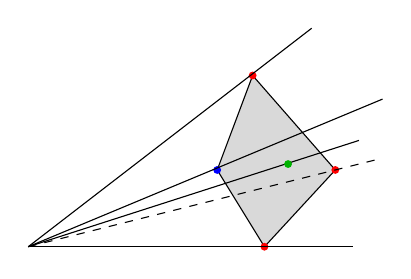
\begin{tikzpicture}[scale=0.75]
		\draw[fill=gray!30] (1.8,2.4) node[fill=red,circle,inner sep=1pt] {} 
			-- (3.2,0.8) node[fill=red,circle,inner sep=1pt] {}
			-- (2,-0.5)  node[fill=red,circle,inner sep=1pt] {}
			-- (1.2,0.8) node[fill=blue,circle,inner sep=1pt] {}
			-- cycle;
		\draw (2.8,3.2) -- (-2,-0.5);
		\draw (-2,-0.5) -- (3.5,-0.5);
		\draw[dashed] (-2,-0.5) -- (4,1);
		\draw (-2,-0.5) -- (4,2);
		\draw (3.6,1.3) -- (-2,-0.5);
		\node[fill=green!70!black,circle,inner sep=1pt] at (2.4,0.9) {};
		\end{tikzpicture}
	\end{center}
	We can use the gray polygon, the intersection of this cone with a hyperplain,
	to represent it, and blow up along the green vector which is the positive
	linear combination of three red vectors, then we can get three new subcones
	as shown in the following diagram.
	\begin{center}
		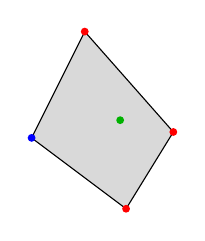
\begin{tikzpicture}[scale=0.75,baseline={([yshift=-.5ex]current bounding box.center)}]
		\draw[fill=gray!30] (2.5,0.2) node[fill=red,circle,inner sep=1pt] {}
			-- (1.6,-1.6) node[fill=blue,circle,inner sep=1pt] {}
			-- (3.2,-2.8) node[fill=red,circle,inner sep=1pt] {}
			-- (4,-1.5) node[fill=red,circle,inner sep=1pt] {}
			-- cycle;
		\node[fill=green!70!black,circle,inner sep=1pt] at (3.1,-1.3) {};
		\end{tikzpicture}
		$\longmapsto$
		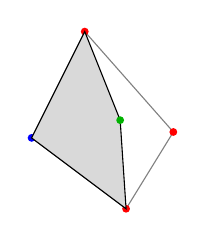
\begin{tikzpicture}[scale=0.75,baseline={([yshift=-.5ex]current bounding box.center)}]
		\draw[gray] (2.5,0.2) node[fill=red,circle,inner sep=1pt] {}
			-- (1.6,-1.6) node[fill=blue,circle,inner sep=1pt] {}
			-- (3.2,-2.8) node[fill=red,circle,inner sep=1pt] {}
			-- (4,-1.5) node[fill=red,circle,inner sep=1pt] {}
			-- cycle;
		\draw[fill=gray!30] (2.5,0.2) -- (3.1,-1.3) -- (3.2,-2.8) -- (1.6,-1.6) --cycle;
		\node[fill=green!70!black,circle,inner sep=1pt] at (3.1,-1.3) {};
		\end{tikzpicture}
		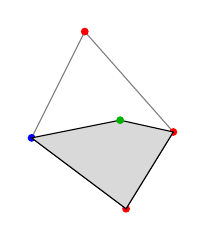
\begin{tikzpicture}[scale=0.75,baseline={([yshift=-.5ex]current bounding box.center)}]
		\draw[gray] (2.5,0.2) node[fill=red,circle,inner sep=1pt] {}
			-- (1.6,-1.6) node[fill=blue,circle,inner sep=1pt] {}
			-- (3.2,-2.8) node[fill=red,circle,inner sep=1pt] {}
			-- (4,-1.5) node[fill=red,circle,inner sep=1pt] {}
			-- cycle;
		\draw[fill=gray!30] (3.1,-1.3) -- (4,-1.5) -- (3.2,-2.8) -- (1.6,-1.6) --cycle;
		\node[fill=green!70!black,circle,inner sep=1pt] at (3.1,-1.3) {};
		\end{tikzpicture}
		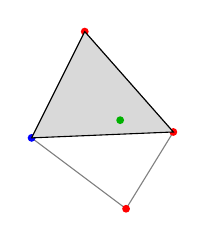
\begin{tikzpicture}[scale=0.75,baseline={([yshift=-.5ex]current bounding box.center)}]
		\draw[gray] (2.5,0.2) node[fill=red,circle,inner sep=1pt] {}
			-- (1.6,-1.6) node[fill=blue,circle,inner sep=1pt] {}
			-- (3.2,-2.8) node[fill=red,circle,inner sep=1pt] {}
			-- (4,-1.5) node[fill=red,circle,inner sep=1pt] {}
			-- cycle;
		\draw[fill=gray!30] (2.5,0.2) -- (4,-1.5) -- (1.6,-1.6) -- (1.6,-1.6) --cycle;
		\node[fill=green!70!black,circle,inner sep=1pt] at (3.1,-1.3) {};
		\end{tikzpicture}
	\end{center}

	%\begin{center}
	%\begin{tikzpicture}
	%\draw (1.7,2.6) -- (-2,-0.5);
	%\draw (-2,-0.5) -- (3.5,-0.5);
	%\draw (-2,-0.5) -- (4.2,1.7);
	%\draw (1.1,2.1) -- (3.6,1.5) -- (2.8,-0.5) -- cycle ;
	%\draw[dashed] (-2,-0.5) -- (3.5,0.9);

	%\draw[dashed] (1.1,2.1) -- (2.7,0.7);
	%\draw[dashed] (3.6,1.5) -- (2.7,0.7);
	%\draw[dashed] (2.8,-0.5) -- (2.7,0.7);
	%\node[fill=green,circle,inner sep=1pt] at (2.7,0.7) {};

	%\fill[opacity=0.1,blue]  (1.1,2.1) -- (-2,-0.5) -- (2.7,0.7);
	%\fill[opacity=0.1,green] (-2,-0.5) -- (2.7,0.7) -- (2.8,-0.5);
	%\fill[opacity=0.1,red] (-2,-0.5) -- (2.7,0.7) -- (3.6,1.5);
	%\end{tikzpicture}	
	%\end{center}
	%we blow up the cone according to the middle vector on the above diagram, and
	%three generated cones form a subdivision of the original cone.

	% However, if $n_j$ is not the vector of a edge of the cone and $\sum_{i\in S} c_i n_i\neq n_j$,
	% then generated cones may have overlaps with each other. In this case, usually we
	% blow up such that $\sum_{i\in S} c_i n_i\neq n_j$ and $j\not\in S$, and we will get cones 
	% without overlaps. What's more, the generated matrices have two identical rows. 
	% Suppose that $n_j=n_k$ in the matrix, it's equivalent to say that the polynomial is the 
	% function of the product $x_jx_k$.
	
	The bonus of this viewpoint is that we can see information of many rounds 
	in only one picture.

	\item If $n^J_i \geq n^I_i$ for all $i$, we can drop column vector $n^J$. Geometrically, 
	it means that the cone spanned by $\{n_i\}$ is in the semi-space defined by $z^J\geq z^I$.
	Thus let's define $H^{IJ}$ as the semi-space defined by $z^I\leq z^J$ in the space of column vectors for future use. Therefore, if we can cut the cone by blowing up into small cones such that 
	each of them is totally contained in some semi-spaces $\{H^{IJ}\}$, then
	the number of columns of generated matrices decreases strictly.

	The possible obstacle to do this is that the intersection of all hyperplains $h^{IJ}=\{z\,:\, z^I=z^J\}$, 
	or equivalently the vector $(1,1,\dots,1)$, 
	is contained in the original cone.
	In this case, no matter how blow-ups `divide' the cone, 
	there always exists a cone contain
	$(1,1,\dots,1)$ so that it is not contained in any semi-space $H^{IJ}$.
    In this case, the number of \emph{columns} rather than the number of rows is reduced.

\item One possible way to `divide' the cone is to reduce the number of outside vertices.
	Before giving the explicit definition of outside or insider, let's first consider a $N=3$ 
	example to show this idea.
	\begin{center}
	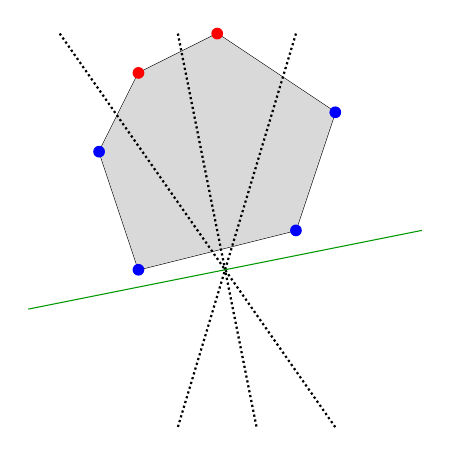
\begin{tikzpicture}
		\draw (2,-1.5) -- (1.5,-2.5) -- (2,-4) -- (4,-3.5) -- (4.5,-2) -- (3,-1) -- cycle;
		\fill[gray!30] (2,-1.5) -- (1.5,-2.5) -- (2,-4) -- (4,-3.5) -- (4.5,-2) -- (3,-1) -- cycle;
		\draw[thick,densely dotted] (1,-1) -- (4.5,-6);
		\draw[thick,densely dotted] (2.5,-1) -- (3.5,-6);
		\draw[thick,densely dotted] (4,-1) -- (2.5,-6);
		\node[circle,inner sep=1.5pt,fill=blue] at (2,-4) {};
		\node[circle,inner sep=1.5pt,fill=blue] at (4.5,-2) {};
		\node[circle,inner sep=1.5pt,fill=blue] at (1.5,-2.5) {};
		\node[circle,inner sep=1.5pt,fill=blue] at (4,-3.5) {};
		\node[circle,inner sep=1.5pt,fill=red] at (2,-1.5) {};
		\node[circle,inner sep=1.5pt,fill=red] at (3,-1) {};
		\draw[green!60!black] (0.6,-4.5) -- (5.6,-3.5);
	\end{tikzpicture}
	\end{center}
In above diagram, the outside vertices are labeled by blue points, and inside vertices are
labeled by red points. If we blow up the cone along a inside vector which is 
the linear combination of outside vertices, then the number of outside
vertices of each subcone is reduced by $1$. Therefore, after finite such operation,
any subcone is contained in some semi-spaces defined by outside hyperplains.

\item 
	In higher dimensional space, hyperplains $h^{IJ}$ divide 
	the whole space $\mathbb R_+^N$ into many small cones which 
	can be labeled by a permutation of $(1,\dots,N)$. 
	For a region label by $\eta$, it's given by the inequality 
	$0\leq z^{\eta_1}\leq \cdots\leq z^{\eta_N}$. 
	
	For a given cone, we can find a hyperplain $H:\hat{n}\cdot z=0$ crossing
	$(1,1,\dots,1)$ (the green line in the above diagram) 
	such that the cone is contained in one side of this hyperplain.
	In other words, we are looking for a vector $\hat{n}\in \mathbb R^N$ 
	such that
	\[
		\sum_{I=1}^N \hat{n}^I=0\quad \text{and}\quad \hat{n}\cdot
		n_i=\sum_{I=1}^N\hat{n}^In^I_i\geq 0 \text{ for all $i$}.
	\]

	Note that, in $N=3$ case, a outside region can cross the hyperplain $H$ 
	but a inside region cannot, so we just generalize it to higher dimension.

	Equivalently, a region is inside if and only if $\hat{n}$ is contained in 
	its dual cone spanned by normal vectors of surrounding hyperplains 
	$\{h^{IJ}\}$. Precisely, 
	for the region $R$ label by a permutation $\eta$,
	its dual cone is spanned by
	\[
		\{\mathbf{b}^I_\eta=\mathbf{e}_{\eta_{I+1}}-\mathbf{e}_{\eta_{I}}
		\,:\, 1\leq I\leq N-1\},
	\]
	where $\mathbf{e}_i\in \mathbb R^N$ is the vector whose $i$-th element 
	is $1$ and the other elements are all zero, then
	the region $R$ is inside if and only if there exist nonnegative numbers
	$\{c_I\}$ such that $\hat{n}=\sum_I c_I\mathbf{b}^I_\eta$.
\end{enumerate}
%
Now our algorithm (for one polynomial) is simple: 
For a given cone $(n^I_i)$,
\begin{enumerate}
	\item[(0).] Define a set of matrices $\mathcal M$ and initialize it 
		to $\{(n^I_i)\}$.
	\item[(1).] Replace any matrix by its reduced matrix. If all matrices
		in the set $\mathcal M$ have only one column or row, 
		the algorithm stops.
	\item[(2).] 
		Look for cones containing $(1,\dots,1)$ in $\mathcal M$.
		If there's no cone containing $(1,\dots,1)$, goto step (3).
		Otherwise, blow up such matrices along $(1,\dots,1)$, 
		add all generated matrix into the set $\mathcal M$ and goto step (1).
	\item[(3).] For each cone in $\mathcal M$, 
		reduce the number of outside vertices by blow-ups 
		such that each generated matrix is totally contained in some 
		semi-spaces $\{H^{IJ}\}$, add all generated matrices into 
		the set $\mathcal M$ and goto step (1).
\end{enumerate}

This algorithm always terminates in finite steps. If we do not want to rescale powers
as the original Hironaka polyhedron game, we may use more steps because in this case 
usually we can only slowly shrink the cone such that outside vertices approach the outside 
hyperplains step by step. However, after finite steps, we can still make sure that 
the number of outside vertices can be reduced, so the algorithm still terminates, but
the algorithm involving rescaling of powers usually is more efficient.

Now let's give a simple example to end this section. Consider the matrix
\[
	M=\left(
		\begin{array}{ccc}
			n_1 \\
			n_2 \\
			n_3
		\end{array}
	\right)
	=\left(
		\begin{array}{ccc}
			0 & 3 & 1 \\
			2 & 0 & 1 \\
			1 & 2 & 0
		\end{array}
	\right),
\]
we can represent the cone by the projection of its intersection with 
the hyperplain $z^1+z^2+z^3=12$ on the $z^1$-$z^2$ plane.
\begin{center}
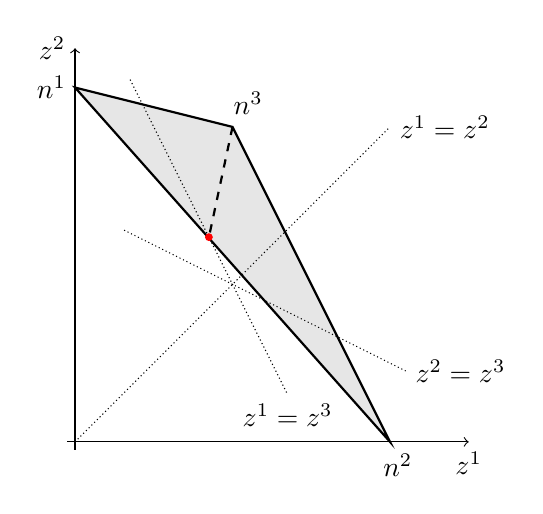
\begin{tikzpicture}
\fill[opacity=0.2,gray] (0,4.5) -- (4,0) -- (2,4) -- cycle ;
\draw[thick] (0,4.5) -- (4,0) -- (2,4) -- cycle ;
\draw[->] (-0.1,0) -- (5,0) node[below] {$z^1$};
\draw[->] (0,-0.1) -- (0,5) node[left] {$z^2$};
\draw[densely dotted] (0,0) -- (4,4) node[right] {$z^1=z^2$};
\draw[densely dotted] (4.2,0.9)  node[right] {$z^2=z^3$} -- (0.6,2.7);
\draw[densely dotted] (0.7,4.6)  -- (2.7,0.6)  node[below] {$z^1=z^3$};
\draw[thick,dashed] (2,4) -- (1.7,2.6) node[circle, fill=red, inner sep=1pt] {};
%\node[red] at (1.6,2.4) {$q$};
\node at (2.2,4.3) {$n^3$};
\node at (4.1,-0.3) {$n^2$};
\node at (-0.3,4.5) {$n^1$};
\end{tikzpicture}
\end{center}
The intersection of three dotted line is the vector $(4,4,4)$, 
so the cone doesn't contain $(1,1,1)$ and we can directly goto step (3).
The outside vertices are $n^1$ and $n^2$, so we first find a inside red point 
as the intersection of the hyperplain 
$z^1=z^3$ and the facet spanned by $\{n^1,n^2\}$ of the cone, 
so in fact the red point represents the vector $n_1+n_2$, 
which tells us that we should blow up $x_1$ and $x_2$.
Therefore, the cone is decomposed into two new cones 
\[
	M\mapsto \biggl\{
		\begin{pmatrix}
			0&3&1\\
			2&3&2\\
			1&2&0
		\end{pmatrix},
		\begin{pmatrix}
			2&3&2\\
			2&0&1\\
			1&2&0
		\end{pmatrix}
	\biggr\}
\] 
by blowing up, and these matrices can be reduced to
\[
	M\mapsto \biggl\{
		\begin{pmatrix}
			0&1\\
			2&2\\
			1&0
		\end{pmatrix}\cong
		\begin{pmatrix}
			0&1\\
			1&0
		\end{pmatrix},
		\begin{pmatrix}
			3&2\\
			0&1\\
			2&0
		\end{pmatrix}
	\biggr\}
\]
because the first one is contained in the semi-space $z^3\leq z^2$
and the second one is contained in the semi-space $z^3\leq z^1$.
It's easy to see that all new cones contain $(1,1)$, so we goto step (1) 
and get
\begin{align*}
	M&\mapsto 
	\biggl\{
		\begin{pmatrix}
			0&1\\
		\end{pmatrix},
		\begin{pmatrix}
			1&0\\
		\end{pmatrix},
		\begin{pmatrix}
			0&1\\
			2&0
		\end{pmatrix},
		\begin{pmatrix}
			3&2\\
			2&0
		\end{pmatrix}
	\biggr\}\\
	 &\cong
	 \biggl\{
		 \begin{pmatrix}
			 0\\
		 \end{pmatrix},
		 \begin{pmatrix}
			 0\\
		 \end{pmatrix},
		 \begin{pmatrix}
			 0&1\\
			 2&0
		 \end{pmatrix},
		 \begin{pmatrix}
			 2\\
			 0
		 \end{pmatrix}
	 \biggr\}\\
	 &\mapsto
	 \biggl\{
		 \begin{pmatrix}
			 0\\
		 \end{pmatrix},
		 \begin{pmatrix}
			 0\\
		 \end{pmatrix},
		 \begin{pmatrix}
			 2&0
		 \end{pmatrix},
		 \begin{pmatrix}
			 0&2\\
		 \end{pmatrix},
		 \begin{pmatrix}
			 2\\
			 0
		 \end{pmatrix}
	 \biggr\}
\end{align*}
Now the algorithm stops. If we go back to the integral of the polynomial $p=y^2z+x^3z^2+xy$
corresponding to $M$, we should carefully add factors $c_i$
corresponding to the change of variables $x_i\mapsto x_i^{1/c_i}$ and we will get $5$ terms 
in above example.
\begin{align*}
	\int_{[0,\epsilon]^3}\frac{\dif x}{x}&\frac{\dif y}{y}\frac{\dif z}{z}
	x^{\alpha' X}y^{\alpha' Y}z^{\alpha' Z}(y^2z+x^3z^2+xy)^{-\alpha' c}\\
	=\,&\frac{1}{{\alpha'}^3}\biggl(
	\frac{1}{X (-2 c+X+Y) (-c+X+Z)}+\frac{1}{Z (-2 c+X+Y) (-c+X+Z)}\\
	&+\frac{1}{Z (-2 c+X+Y) (-3 c+X+2 Y)}+
	\frac{2}{Z (-3 c+X+2 Y) (-2 c+2 Y+Z)}\\
	&+\frac{2}{2 Y (-3 c+X+2 Y) (-2 c+2 Y+Z)}
	\biggr) +O({\alpha'}^{-2}).
\end{align*}

%Empirically, we can use a simplified version of this algorithm to choose $S$ for player A.
%For a given matrix, if player A chooses $S$ such that 
%\begin{compactenum}[\quad\, 1)]
%\item $\sum_{i\in S} n_i^I>0$ for all $I$;
%\item $\sum_{i\in S} n_i$ has maximal number of minimals;
%\item $\#S$ is minimal,
%\end{compactenum}
%then he/she can still win in all cases we have tested. 
%This strategy doesn't contain any transformation like $x_i\mapsto x_i^{1/c_i}$. The first 
%condition means that the polynomial goes to zero when $x_i\to 0$ for $i\in S$, and
%the last is used to avoid too many vertices. These two condition is first
%introduced in \cite{Binoth:2000ps}, and called strategy X in \cite{bogner2009mathematical}.
%Here, we introduce one more condition $2)$, which may be the key condition to avoid 
%infinite iteration. It's used to make sure the vector $\sum_{i\in S} n_i$
%is choosen on some hyperplains $z^I=z^J$.

%It's not clear now whether the simplified version is a winning strategy,
%but it's more efficient than lots of well-known winning strategies, and it's 
%very easy to code.


% \section{Scattering-Equation Map}
 
% \begin{defi}[Convex Hull]
% The convex hull of a set of vectors $\{\mathbf n^I\,:\, I\in \mathscr A\}$ is defined by
% \[
% 	\operatorname{ConvexHull}\bigl(\{\mathbf n^I\,:\, I\in \mathscr A\}\bigr)
% 	:=\Biggl\{\sum_{I\in\mathscr A}\lambda_I \mathbf n^I\,:\,
% 	\text{$\lambda_I\geq 0$ and $\sum_I\lambda_I=1$}\Biggr\},
% \]
% if $\mathscr A$ is a infinite set, we further require that in each summation, 
% only finite $\lambda_I$ don't vanish.
% \end{defi}

% \begin{defi}[Newton Polytope]
% For a subtraction free Laurent polynomial 
% \[
% 	f = \sum_{I\in \mathscr A} a_I \prod_{i=1}^n x_i^{n^I_i},
% \]
% we define the Newton polytope of $f$ by
% \[
% 	N(f)=\operatorname{ConvexHull}\bigl(\{\mathbf n^I\,:\, I\in \mathscr A\}\bigr),
% \]
% where $\mathbf n^I=(n^I_1,\dots,n^I_n)$. 
% \end{defi}
% 
% \begin{defi}[Minkowski Sum]
% Minkowski sum of two subsets $A$ and $B$ of $\mathbb R^n$ is defined by 
% \[
% 	A+B=\{x+y\,:\,x\in A,\, y\in B\}.
% \] 
% \end{defi}
% 



\section{Conclusions and Outlook}


In this article, we have shown how to obtain the leading order contribution of stringy integrals by a blow-up algorithm. These integrals are generations of tree-level scattering of open strings and provide natural $\alpha'$-deformed canonical forms for general polytopes.  Interestingly, the algorithm is equivalent to a winning strategy for a simplified version of Hironaka's polyhedra game since more moves can be taken in our case.

All information about the leading order of such integrals is contained in the Minkowski sum $N_{P}$ of Newton polytopes of the regulating polynomials. In this sense, the blow-up method gives a way to reconstruct the polytope $N_{P}$ from its vertices. However, as we saw in section 3, spurious poles and hence spurious vertices are produced in the process of blow-ups. Additional efforts are still needed to recognize the real poles and vertices, especially when the dimensionality increases (curse of dimensionality) and the regulating polynomials get more and more complicated. The result obtained by blowing up is correct but redundant, thus a interesting question is how the polytope $N_{P}$ emerges form this (usually tedious) result. 


Another way to reconstruct $N_{P}$ is, along with the opposite direction, to find the facets of $N_{P}$ by using the scattering-equation map. Where the aim is to find all directions such that $\mathbf{X}$ approaches facets of $N_{P}$ as $\mathbf{x}$ approaches boundaries of $\mathbb{R}^{D}$ along with these directions~\cite{}. It would be interesting to find any relations between the reconstruction from the bottom up, the blow-up, and the reconstructiong from the top down, the scattering-equation map.

As we saw in section 2, lots of terms have been dropped during the process of blow-ups, while higher order contributions of such integrals with respect to $\alpha'$ certainly depend on the details of regulating polynomials. One way to obtain the higher order contribution is to expand the integrand with respect to $\alpha'$ then integration, the obstacle to this expansion is singularities in poles. The blow-up procedure provide a way to remove this obstacle: each integration region produced by blow-ups only meets singularities of the canonical form at one vertex, then a subtractation can be easily made such that the integrand have no divergence in the integration region.

(Relation with sector decomposition...)



%\appendix

%\section{Proof of bijectivity of the scattering-equation map}
%In section 2, we find that the blowing up procedure is simplified by the fact that the leading order contribution of stringy integrals are given by the canonical function for $N_{P}$, which is the Minkowski sum of Newton polytopes of polynomials forming the regulator. This fact is equivalent to say that the scattering-equation map is a bijection~\cite{}. Here we give another proof for this proposition. 

%\begin{pro*}
	%For a product of $M$ polynomials $P=\prod_{j=1}^M p_j^{\alpha_j}$, 
	%where $\alpha_j>0$, 
	%$p_j=\sum_{I_{j}} a_{{I_j}} x^{\mathbf{n}^{I_j}}$ are polynomials with non-negative coefficients $a_{I_j}$ and
	%\[
		%x^{\mathbf{n}^{I_j}}:=\prod_{i=1}^D x_i^{n^{I_j}_i},
	%\]
	%we define a polytope $N_P$ in $\mathbb R^D$ as the Minkowski sum $N_P=\sum_j \alpha_j N(p_j)$ of Newton polytopes $N(p_j)$.
	%Then the scattering map:
	%\[
		%\mathbf{X}=\frac{\partial \log P}{\partial \log \mathbf{x}},
	%\]
	%where $\mathbf{X}=(X_{1},\ldots,X_{D})$ and $\mathbf{x}=(x_{1},\ldots,x_{D})$, is a one-to-one map from $(0,\infty)^D$ to the interior of $N_P$ when matrix $(n_i^I)$ has full rank%
	%\footnote{When matrix $(n_i^I)$ doesn't have full rank, the map is not one-to-one. 
		%But in fact, we only care about the case that it has full rank, so that $\dim (N(p))=D$. 
		%% If not, there exist some $\mathbf s\neq 0$ such that $\mathbf s \cdot \mathbf n^I=0$ for all $I$. 
		%% In this case,
		%% \[
		%% \mathbf s\cdot\mathbf X=\mathbf s\cdot\frac{\partial \log p}{\partial \log \mathbf x}=0.
		%% \]
		%% Therefore, one can project $\operatorname{im}(\mathbf X)$ 
		%% by setting some $x_i=1$ so that the new matrix $(n^I_i)$ has full rank.	
		%% In this case, one can recover the original image by solving these equations $\mathbf s\cdot\mathbf X=0$
		%% after working out the image in lower dimension.
		%}%
		%. 
	%\end{pro*}
	
	%\begin{proof}
	%The proof is finished in two steps:
	%\paragraph{Step 1: $M=1$}
	%Consider a polynomial $p=\sum_{I} a_I x^{\mathbf n^I}$ with $a_I\geq 0$ for all $I$. 
	%The scattering map now becomes
	%\[
		%\mathbf X(\mathbf{x})=\frac{\partial \log p}{\partial \log \mathbf x}.
	%\]
	%The proposition is equivalent to the claim that the equation $\mathbf X(\mathbf{x})=\mathbf\Lambda$ has a unique solution in $\mathbb R^D$ 
	%if and only if $\mathbf\Lambda\in (N(p))^\circ$. 
	
	%Let $\mathbf{\Lambda}$ be an interior point in $N(p)$ given by 
	%\[
		%\mathbf \Lambda=\sum_{I}\lambda_I\mathbf n^I
		%=\frac{\partial}{\partial \log \mathbf x}\sum_{I}\lambda_I \log x^{\mathbf n^I}
	%\]
	%where $\sum_I \lambda_I=1$ and $\lambda_I > 0$. The equation $\mathbf X(x)=\mathbf \Lambda$ becomes
	%\[
	%\begin{aligned}
		%0=\frac{\partial }{\partial \log \mathbf x}\left(
			%\log p-\sum_{I}\lambda_I \log x^{\mathbf n^I}
		%\right)=\frac{\partial }{\partial \log \mathbf x}\left(
		%\log F(\mathbf x)
		%\right)=\frac{1}{F(\mathbf x)}\frac{\partial F(\mathbf x)}{\partial \log \mathbf x}
	%\end{aligned}
	%\]
	%where
	%\[
		%F(\mathbf x)=\biggl(\sum_I a_I x^{\mathbf{n}^I}\biggr)\prod_J (x^{-\mathbf n^J})^{\lambda_J}.
	%\]
	%or in terms of $\mathbf y=\log \mathbf x$, 
	%\[
		%F(\mathbf y)
		%=\sum_I a_I \exp\left(\mathbf{y}\cdot \left(\mathbf{n}^I-\mathbf{\Lambda}\right)\right).
	%\]
	%Therefore we only need to show that $F(\mathbf y)$ has a unique saddle points in $\mathbb R^D$ 
	%because $F>0$ for all $\mathbf y$.
	
	%To see it, we first notice that $F(\mathbf y)$ is a strict convex function of $\mathbf y$. In fact, the Hessian of $F(\mathbf y)$ is 
	%\[
		%H_{ij}(\mathbf y)=\frac{\partial^2}{\partial y_i\partial y_j}F(\mathbf y)=\sum_I a_I \exp\left(\mathbf{y}\cdot \left(\mathbf{n}^I-\mathbf{\Lambda}\right)\right)\left(\mathbf{n}^I-\mathbf{\Lambda}\right)_i\left(\mathbf{n}^I-\mathbf{\Lambda}\right)_j.
	%\]
	%For any $\mathbf v\neq 0$, 
	%\[
		%\sum_{i,j}v_iv_jH_{ij}=\sum_I a_I \exp\left(\mathbf{y}\cdot \left(\mathbf{n}^I-\mathbf{\Lambda}\right)\right) \left(\mathbf v\cdot (\mathbf{n}^I-\mathbf{\Lambda})\right)^2 >0.
	%\]
	%It cannot vanish because that it only happens when $\mathbf v\cdot (\mathbf{n}^I-\mathbf{\Lambda})=0$ 
	%for all $I$. However, we have assumed $\{\mathbf n^I\}$ has full rank, so
	%vectors $\{\mathbf{n}^I-\mathbf{\Lambda}\}$ span the whole space 
	%$\mathbb R^D$. 
	
	%For a strict convex function $F(\mathbf y)$ on $\mathbb R^D$, it has a unique minimal in $\mathbb R^D$ 
	%if and only if it does not take the minima when $\mathbf{y}$ goes to infinity along any direction. 
	%To this end, we only need to show that there exist some $I$ such that $\mathbf{y}'\cdot (\mathbf{n}^I-\mathbf{\Lambda})>0$ for any $\mathbf{y}'\neq 0$ and $\mathbf\Lambda \in (N(p))^\circ $, which is directly followed from the convexity of $N(p)$: If $\mathbf\Lambda \in (N(p))^\circ$, for a given $\mathbf{y}'\neq 0$, the hyperplain $L$ with normal vector $\mathbf{y}'$ crossing $\mathbf \Lambda$ 
	%divides the space $\mathds{R}^{D}$ into semi-spaces $L^+$ and $L^-$, then any $\mathbf{n}^I$ 
	%in $L^+$ are desired.

	
	%\begin{center}
		%\begin{tikzpicture}
		%\draw[black,thick](3.5,0.5)--(1,0)--(0,-3)--(1.5,-4.5)--(4.5,-3.5)--(5,-1)--cycle;
		%\draw[black,dashed](-1.4,-2)--(6,-2);
		%\draw[->,black,thick](2,-2)--(2,-1);
		%\draw[->,black,thick](2,-2)--(1,0);
		%\node at (2,-2.2) {$\mathbf{\Lambda}$};
		%\node at (2.2,-0.8) {$\mathbf{y}'$};
		%\node at (6.4,-2) {$L$};
		%\node at (5.6,-1.6) {$L^+$};
		%\node at (5.6,-2.4) {$L^-$};
		%\node at (0.6,0) {$\mathbf{n}^I$};
		%\end{tikzpicture}
	%\end{center}
	%Conversely, if $\mathbf\Lambda \not\in N(p)$, one can find a hyperplain $L$ such that $N(p)\subset L^-$, 
	%then the normal vector $\mathbf{y}'$ of $L$ belonging to $L^{+}$ gives the wanted direction since such that $F(t\mathbf{y}')\to 0$ as $t\to \infty$. Hence, $F(\mathbf y)$ has no saddle point in $\mathds{R}^D$ as a positive convex function.
	
	%Therefore, we have proven that $F(\mathbf y)$ has a unique minimal in $\mathbb R^D$ when 
	%$\mathbf \Lambda \in (N(p))^\circ$ and no saddle point in $\mathbb R^D$ when 
	%$\mathbf \Lambda \not\in N(p)$, which proves the first part.
	
	%\paragraph{Step 2: Generic $M$} Let $\mathbf{\Lambda}$ be a interior point in Minkowski sum $\sum_j \alpha_j N(p_{j})$ corresponding to $P=\prod_j p_{j}^{\alpha_{j}}$ given by 
	%\[
		%\mathbf{\Lambda}
		%=\sum_j \alpha_j \mathbf{\Lambda}_j
		%=\sum_j \alpha_{j} \biggl(\sum_{I_j}\lambda_{I_j}\mathbf{n}^{I_j}\biggr)
		%=\frac{\partial}{\partial \log \mathbf{x}}\sum_{j}\alpha_j\biggl( \sum_{I_j}\lambda_{I_j} \log x^{\mathbf n^{I_j}}\biggr)
	%\]
	%where $\sum_{I_j} \lambda_{I_j}=1$ and $\lambda_{I_j} > 0$. Then the equation $\mathbf{X}(\mathbf{x})=\mathbf{\Lambda}$ is 
	%\[
		%0=\frac{\partial }{\partial \log \mathbf{x}}\left(
			%\log P-\sum_{j}\alpha_j\sum_{I_j}\lambda_{I_j} \log x^{\mathbf n^{I_j}}
		%\right)=\frac{\partial }{\partial \log \mathbf{x}}\left(
		%\log \left(\prod_j F_{j}^{\alpha_{j}}\right)
		%\right),
	%\]
	%where
	%\[
		%\begin{aligned}
			%F_j(\mathbf y)&=\sum_{I_{j}} a_{I_{j}} \exp\left(\mathbf{y}\cdot \left(\mathbf{n}^{I_j}-\mathbf{\Lambda}_j\right)\right).
		%\end{aligned}
	%\]	
	%We only need to show that
	%\[
		%F(\mathbf y)=\prod_j F_j(\mathbf{y})^{\alpha_j}	
	%\]
	%has a unique saddle point in $\mathds{R}^D$.
	
	%Here $F(\mathbf y)$ is not necessarily a strict convex function. However, consider a new function
	%\[
		%F(\mathbf y)^{1/\alpha_0}=\prod_j F_j(\mathbf y)^{\alpha_j/\alpha_0},
	%\]
	%where $\alpha_0$ is a positive number such that $\alpha_0< \alpha_j$ for all $j$, which is a convex function 
	%since each factor $F_{j}^{\alpha_{j}/\alpha_{0}}$ is a convex function. Since $F(\mathbf y)^{1/\alpha_0}$ takes its minimum at same points as $F(\mathbf y)$, 
	%we can further assume that $F(\mathbf y)$ is a strict convex function (\textcolor{red}{C: Why?}). 
	
	%Finally, we claim that $F(\mathbf y)$ does not take minimum when $\mathbf{y}$ goes to infinity 
	%along any direction. It is because that for a given $\mathbf{y}$ and each $j$, $F_j(t\mathbf{y})\to \infty$ when $t\to \infty$,
	%so does $F(t\mathbf{y})=\prod_j F_j(t\mathbf{y})^{\alpha_j}$. Therefore, the equation $\mathbf{X}(x)=\mathbf{\Lambda}$ has a unique solution.
	%\end{proof}
	









% \begin{align*}
% 	&\frac{1}{(a+c+2 d-X) (b+c+d-Y)}+\frac{1}{Y (a+c+2 d-X)}+\frac{1}{(b+c+d-Y) (2 b+c+X-2 Y)}\\
% &+\frac{1}{(b+X-Y) (2 b+c+X-2 Y)}+\frac{1}{X (b+X-Y)}+\frac{1}{X Y}
% \end{align*}

\bibliographystyle{unsrt}
\bibliography{main}

\end{document}
